\pagebreak
\section{Discussion}
In this ``Discussion'' section, I first briefly summarize the results. Then I discuss the model features by comparing them with nature observations.

\subsection{Summary of Results}
\begin{figure}[H]
  \centering
    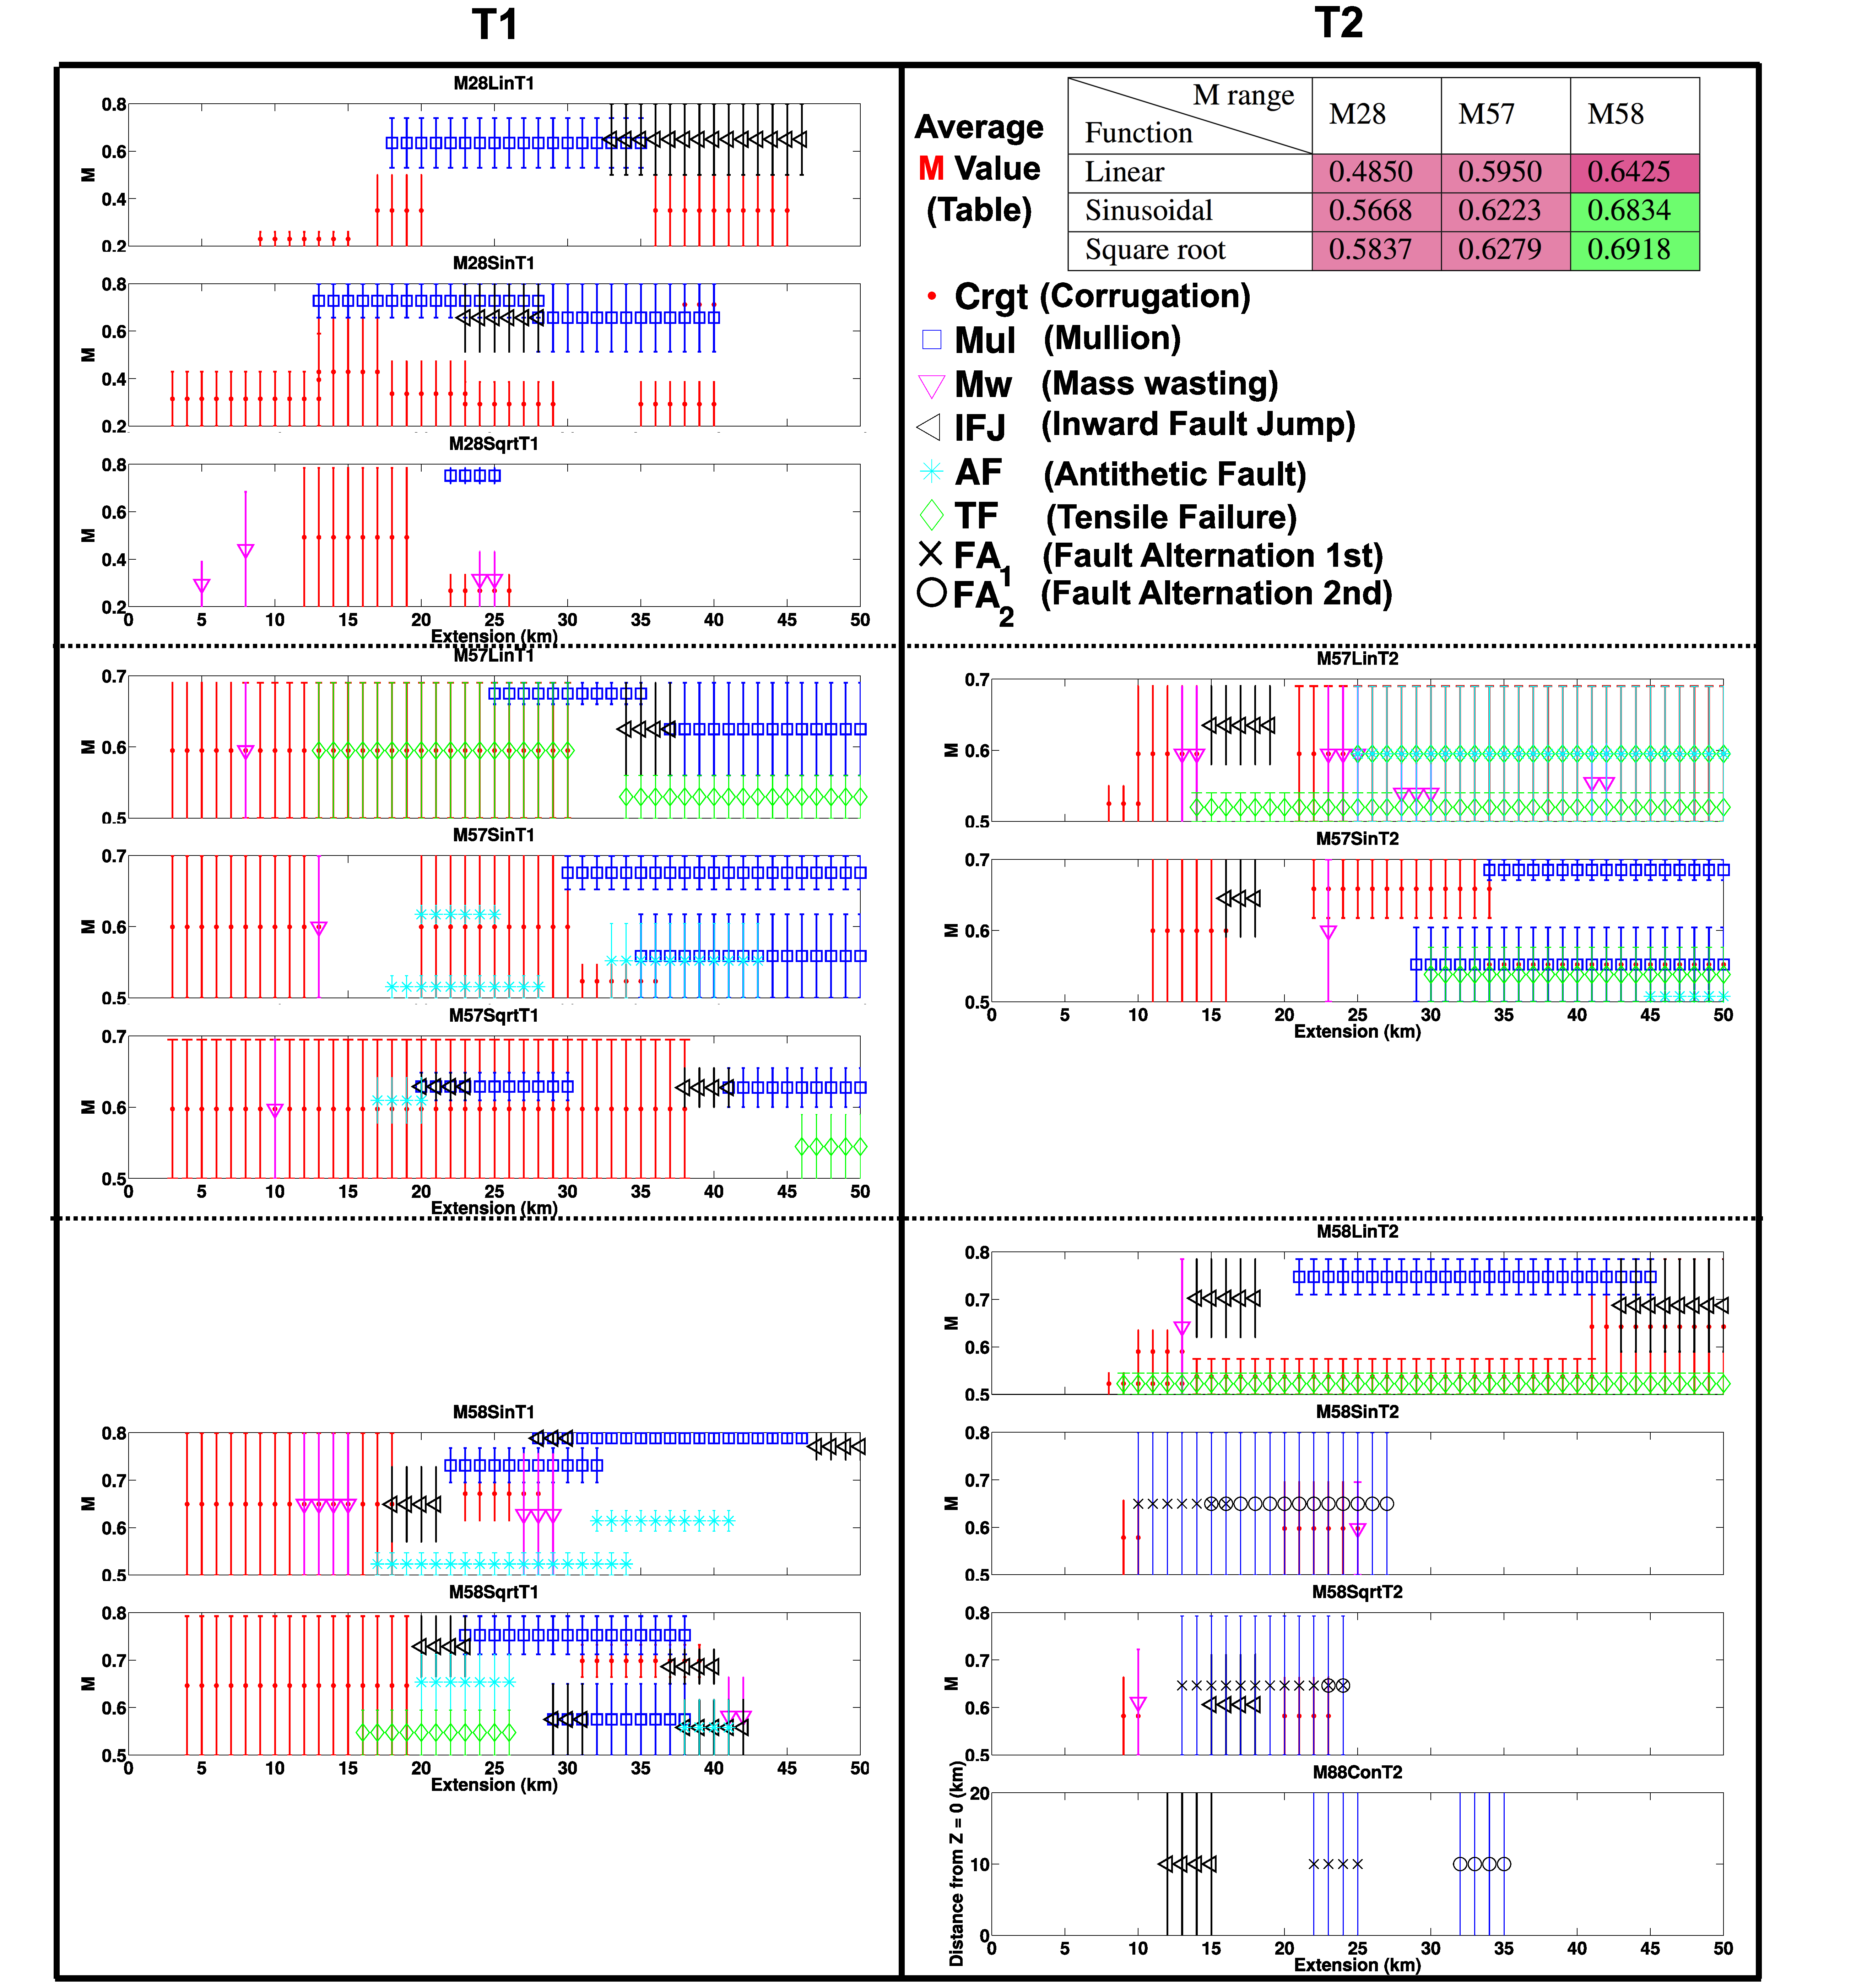
\includegraphics[width=1.05\textwidth]{./Figures/fig_Discussion_Result_Summary_1_Combine_together.eps}
  \caption{Results summary. Model evolution with increasing plate extension.}
 \label{fig_Discussion_Result_Summary_1_Combine_together}
\end{figure}   

Model results show systematic changes when the average M value ($\bar{M}$) increases. $\bar{M}$ is the value of integration of M along the ridge divided by the length of the ridge segment. As seen in the table of Figure~\hyperref[fig_Discussion_Result_Summary_1_Combine_together]{\ref{fig_Discussion_Result_Summary_1_Combine_together}}, $\bar{M}_{M58} > \bar{M}_{M57} > \bar{M}_{M28}$ and within each M range, $\bar{M}$ for functional form with sqaure root is higher than that for sinusoidal and linear. 

Comparing the models with slower weakening rate (type 1) (left column of Figure~\hyperref[fig_Discussion_Result_Summary_1_Combine_together]{\ref{fig_Discussion_Result_Summary_1_Combine_together}}), when $\bar{M}$ increases, faulting (i.e. inward fault jump, antithetic fault) as well as other main model behaviors (i.e. corrugation, mullion, mass wasting, tensile failure) become more complex and dynamical with higher recurrence ferquencies.

Comparing M28SinT1 and M28LinT1 shows that the inward fault jump for M28SinT1 (with higher $\bar{M}$) happens earlier and lasts a shorter period of time. As $\bar{M}$ increases to 0.5837 for M28SqrtT1, mass wasting first shows up. During the mass wasting, a curved fault scarp with $\sim$1 km relief is produced and it has a shape very similar to 13 $\degree$N, Mid-Atlantic Ridge (please refer to a detailed discussion in the next section). 

When M57 are compared to M28 models, corrugations show up earlier along the whole 20 km ridge segment. All three models have mass wasting. For M57LinT1 ($\bar{M} =$ 0.5950), it begins to have tensile failure which releases tensional stress in the hanging wall and results in the delay of inward fault jump. For M57SinT1 ($\bar{M} =$ 0.6223), antithetic fault first shows up and together with mass wasting lead to the absence of inward fault jump. The antithetic fault at the lower M side helps to maintain a closer to ridge axis termination which results in a larger mullion struc(Figure~\hyperref[fig_Discussion_Observation_1_Tucholke1998]{\ref{fig_Discussion_Observation_1_Tucholke1998}.a})ture at the lower M side and thus produces an OCC with a shape similar to the Atlantis Massif at 30 $\degree$N Mid-Atlantic Ridge. For M57SqrtT1 ($\bar{M} =$ 0.6279), it has twice of inward fault jumps and each of them produces a curved toward ridge axis termination. The curved termination is responsible for the following small scale mullion structure.
   
Comparing M58 and M57 models shows that the two M58 models have 3 and 4 times of inward fault jump respectively while M57 models have at most twice of that. Also, corrugations of M57 show up earlier and it might imply that corrugation favors specific range of $\frac{\partial M}{\partial Z}$, neither too higher, nor too low. Between M58SinT1 ($\bar{M} =$ 0.6834) and M58SqrtT1 ($\bar{M} =$ 0.6918), the major difference is M28SqrtT1 has twice inward fault jumps at the lower M side because M values are higher at the lower M side.

When comparing models with different weakening rate (type 1 versus type 2), the most obvious difference is that only two of type 2 models with $\bar{M} >$ 0.6425 generates alternating faults, they are M58SinT2 and M58SqrtT2. They don't have mullion structure because the high frequency of fault alternation allows a specific pattern of termination to last only for a shorter period of time. Also, they neither have tensile failure nor antithetic fault. Note that M58LinT2 ($\bar{M} =$ 0.6425) does not generate fault alternation and it indicates that not only the range of M (M58) but also the average M value along the ridge $\bar{M}$ are responsible for the fault alternation. This provides an upper limit in our 3D models for producing long lasting detachment fault that can generate OCCs. Comparing M57T2 and M57T1 models shows that M57T2 models generally have earlier inward fault jump but later corrugations. For the model with constant M = 0.8 along the ridge axis, the inward fault jump and fault alternations have a period of $\sim$10 km of extension. Corrugation, mullion structures, mass wasting, antithetic fault and tensile failure are not produced in this model which implies that varying M is necessary for producing those features.

\begin{figure}[h]
 \centering
  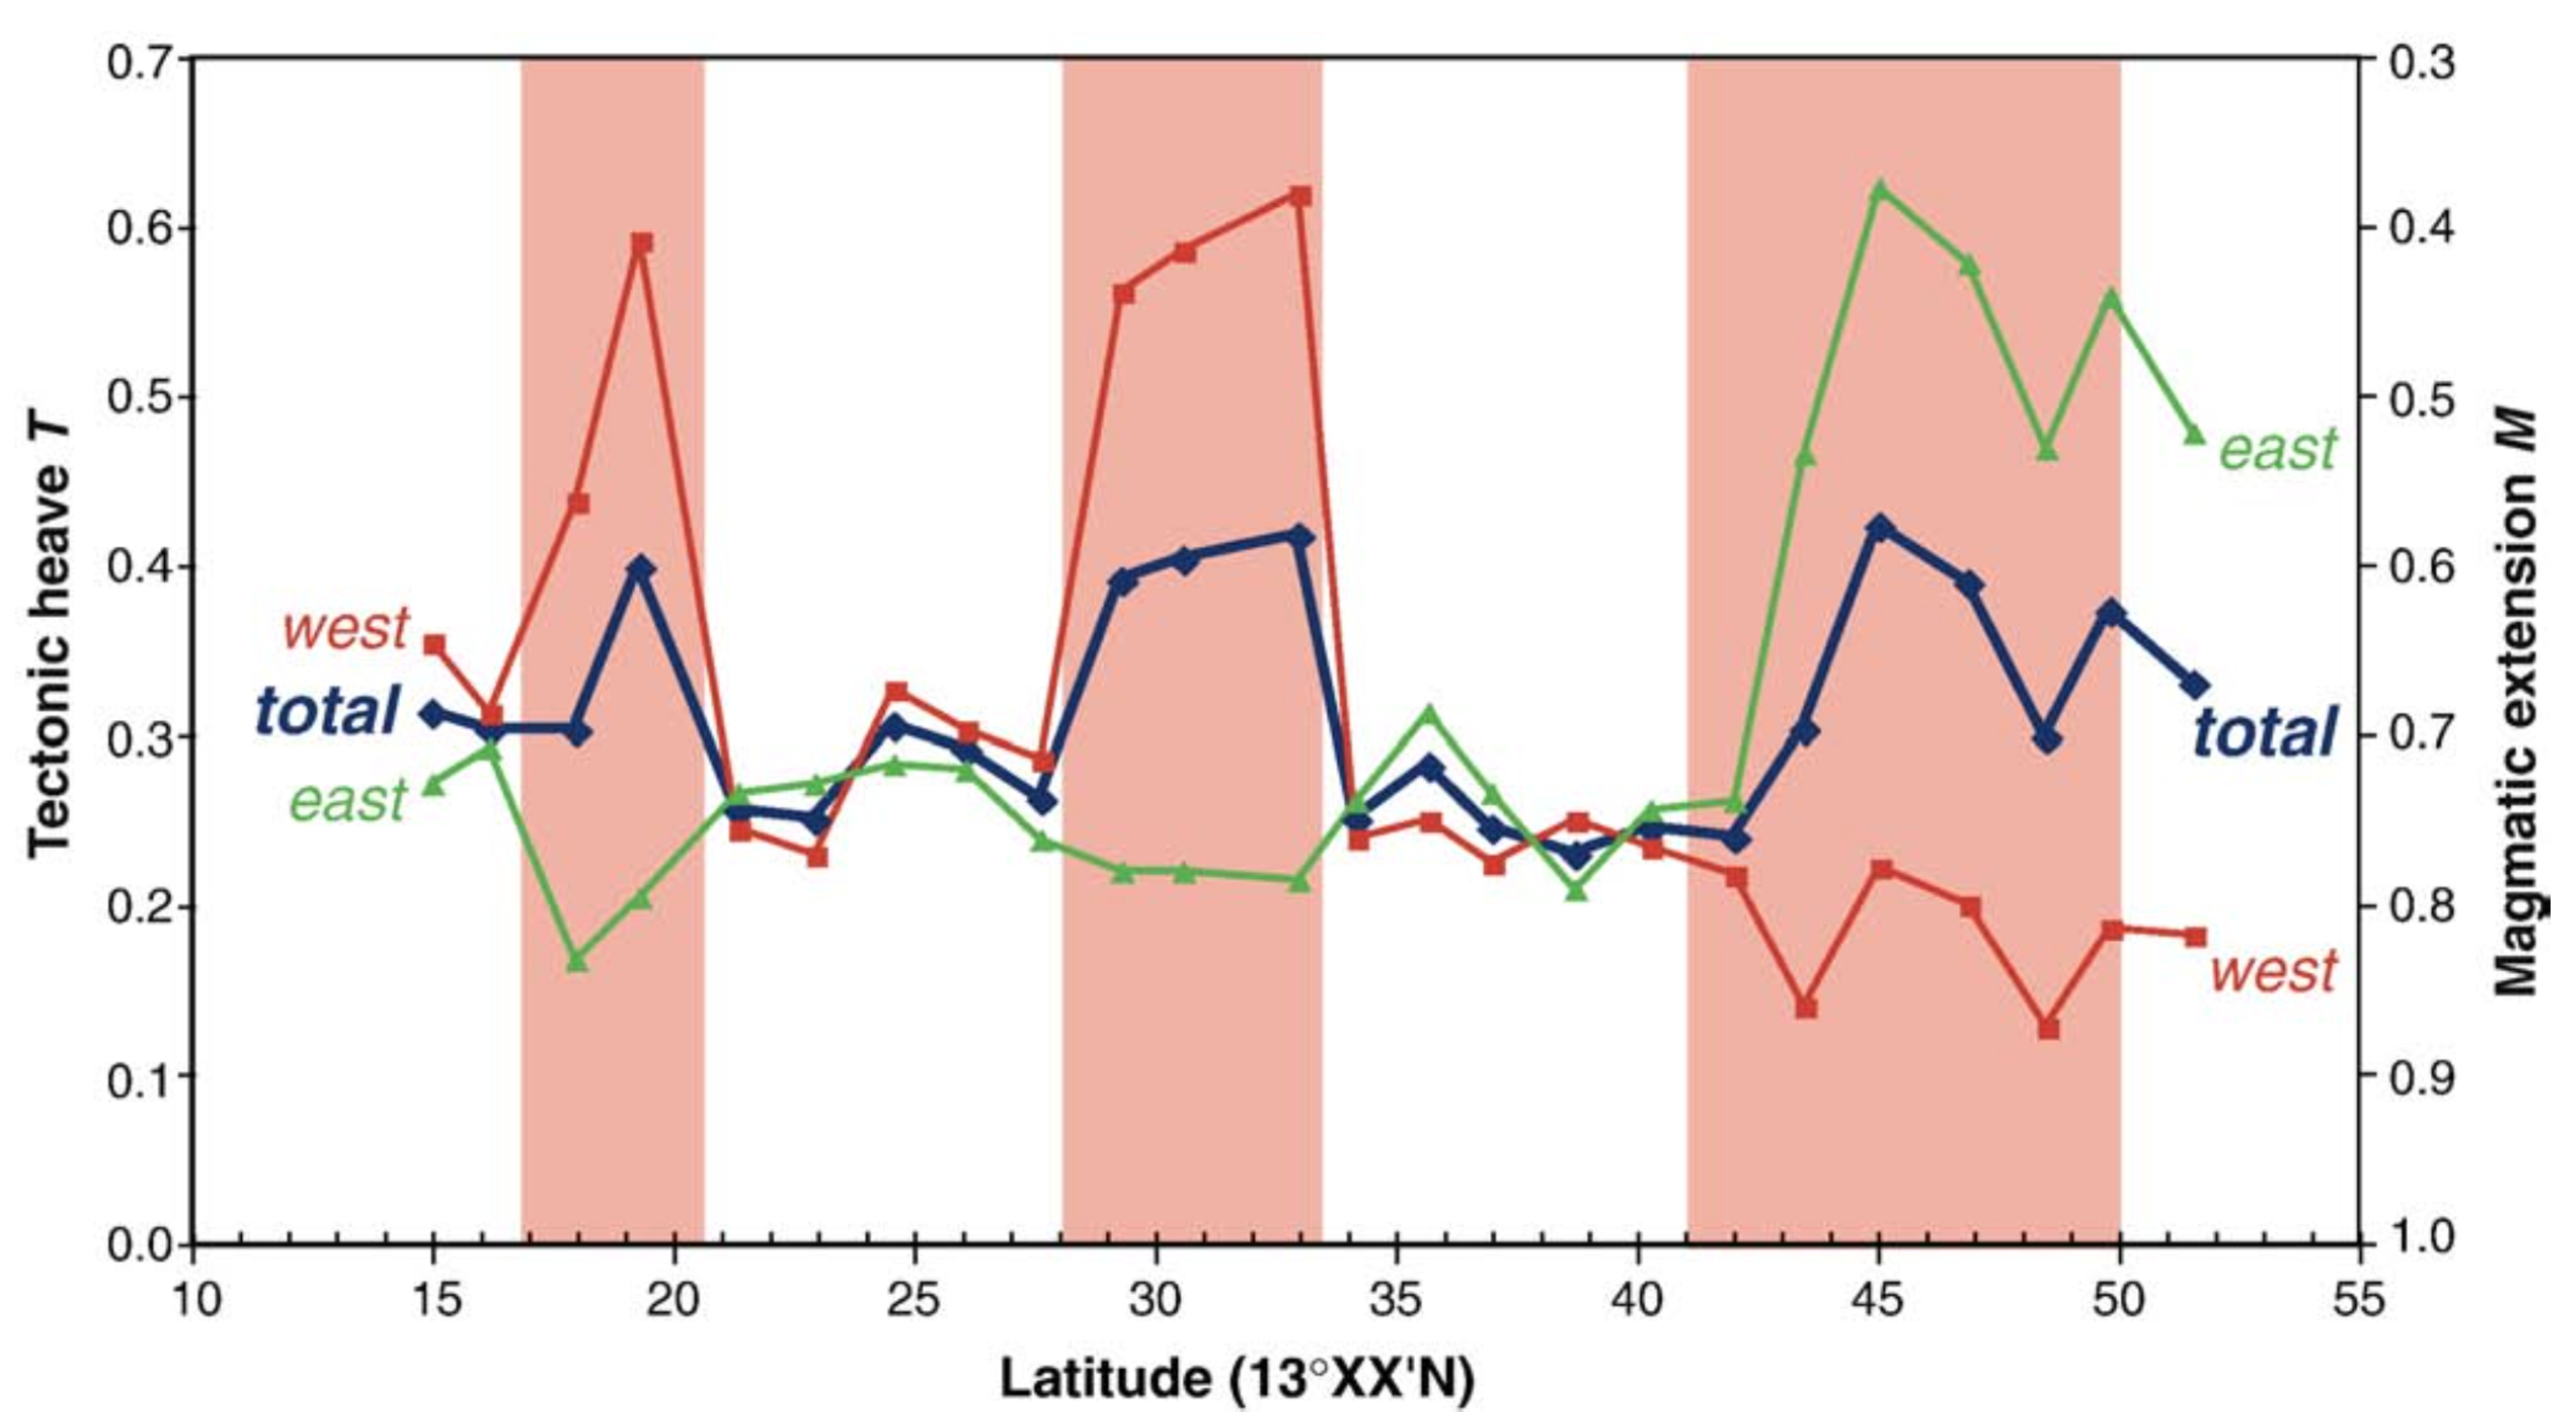
\includegraphics[width=1\textwidth]{./Figures/fig_Discussion_ResultsSummary_MacLeod2009.eps}
 \caption{Along-axis variations in total accumulated tectonic heave T in the past 1.86 Ma (since chron C2n), and consequent inferred magmatic component M (= 1 $-$ T) as a proportion of total plate separation (blue line). Pink shaded areas delineate loci of the active or recently active OCCs. The relative contributions of tectonic strain from the western and eastern flanks of the axis that give rise to the total heave T are shown by red and green lines respectively. Adapted from \citep{MacLeod2009}. }
 \label{fig_Discussion_ResultsSummary_MacLeod2009}
\end{figure}

In addition, the upper limit of $\bar{M} = $ 0.6425 for allowing a long lasting detachment fault to produce an OCC in our model is consistent to the results from a near-bottom sidescan bathymetric profiler survey and sampling study of the Mid-Atlantic Ridge near 13 $\degree$N \citep{MacLeod2009}. As shown in Figrure~\hyperref[fig_Discussion_ResultsSummary_MacLeod2009]{\ref{fig_Discussion_ResultsSummary_MacLeod2009}}, the average M value $\bar{M} =$ 0.63 $\pm$ 0.05 for the pink area where OCCs are present while when there is no OCC, $\bar{M} =$ 0.73 $\pm$ 0.03.

Under similar physical condition of our model setup (e.g. thermal structure, rheology relationship, spreading velocity, weakening rate), the upper limit of $\bar{M} = $ 0.6425 predicts a boundary value between two observed morphology end members for slow spreading ridges: 1) long wavelength OCCs generated by asymmetric spreading on the detachment fault; 2) high frequency abyssal hills results from symmetric spreading of alternating high angle normal faults. Although the number of $\bar{M} = $ 0.6425 is highly consistent with natural observation (e.g. \citep{MacLeod2009}), we still need more works for a comprehensive result because model parameter such as viscosity of the underlying asthenosphere also contributes to whether fault alternates. For example, \citep{Allken2012} shows that higher value of viscosity of the ductile asthenosphere leads to better coupling between crust and mantle and promotes distributed muliple faulting rather than a focused long-lived detachment fault.

Previous 2D studies suggest that OCCs are most likely to form when M = 0.3 $\sim$ 0.5 [\citealp{Buck2005};\citealp{Tucholke2008}]. However, conflicts exist between model prediction and nature observation in both the upper and lower limits. For the upper limit conflict that OCCs are observed with M $>$ 0.5, \citet{Olive2010} suggests an explanation from a 2D model study that magma supplied in the ductile lower crust and upper mantle will not affect the faulting pattern and thus allows OCCs to be created under excessive diking. However, our 3D model results provides an alternative explanation that due to the along ridge coupling (i.e. torsion and shear), the region (M = 0.3 $\sim$ 0.5) along the ridge that promotes stable spreading by detachment faulting helps maintain the normal fault outside the region along the ridge. Once the detachment fault initiates along the whole ridge segment, it is very hard to modify the faulting pattern especially for a faster weakening rate (type 1). Thus, the detachemnt fault at the higher M side (M $>$ 0.5) can still last for more than 20 km of plates separation (Figure~\hyperref[fig_Discussion_Result_Summary_1_Combine_together]{\ref{fig_Discussion_Result_Summary_1_Combine_together}}) before the fault alternation or inward fault jump ceases the exhuming process of the ultramafic mantle rocks. This along ridge coupling can also be used to explain the conflict at the lower limit end when OCC is produce with observed M $<$ 0.3 (e.g. \citealp{Dick2008}; \citealp{Grimes2008} and \citealp{Baines2008}). This along ridge coupling is also able to explain why our 3D result for the upper limit of $\bar{M} = $ 0.6425 is higher than previous 2D studies of M = 0.3 $\sim$ 0.5 [\citealp{Buck2005};\citealp{Tucholke2008}]. 


\subsection{Comparing model results with nature observation}

In this section, I will compare the model behaviors with nature observation in terms of the following model produced features: inward fault jump, fault alternation, mass wasting, hourglass shape median valley, mullion structure and corrugation.

\subsubsection{Inward fault jump}
\begin{figure}[h]
 \centering
  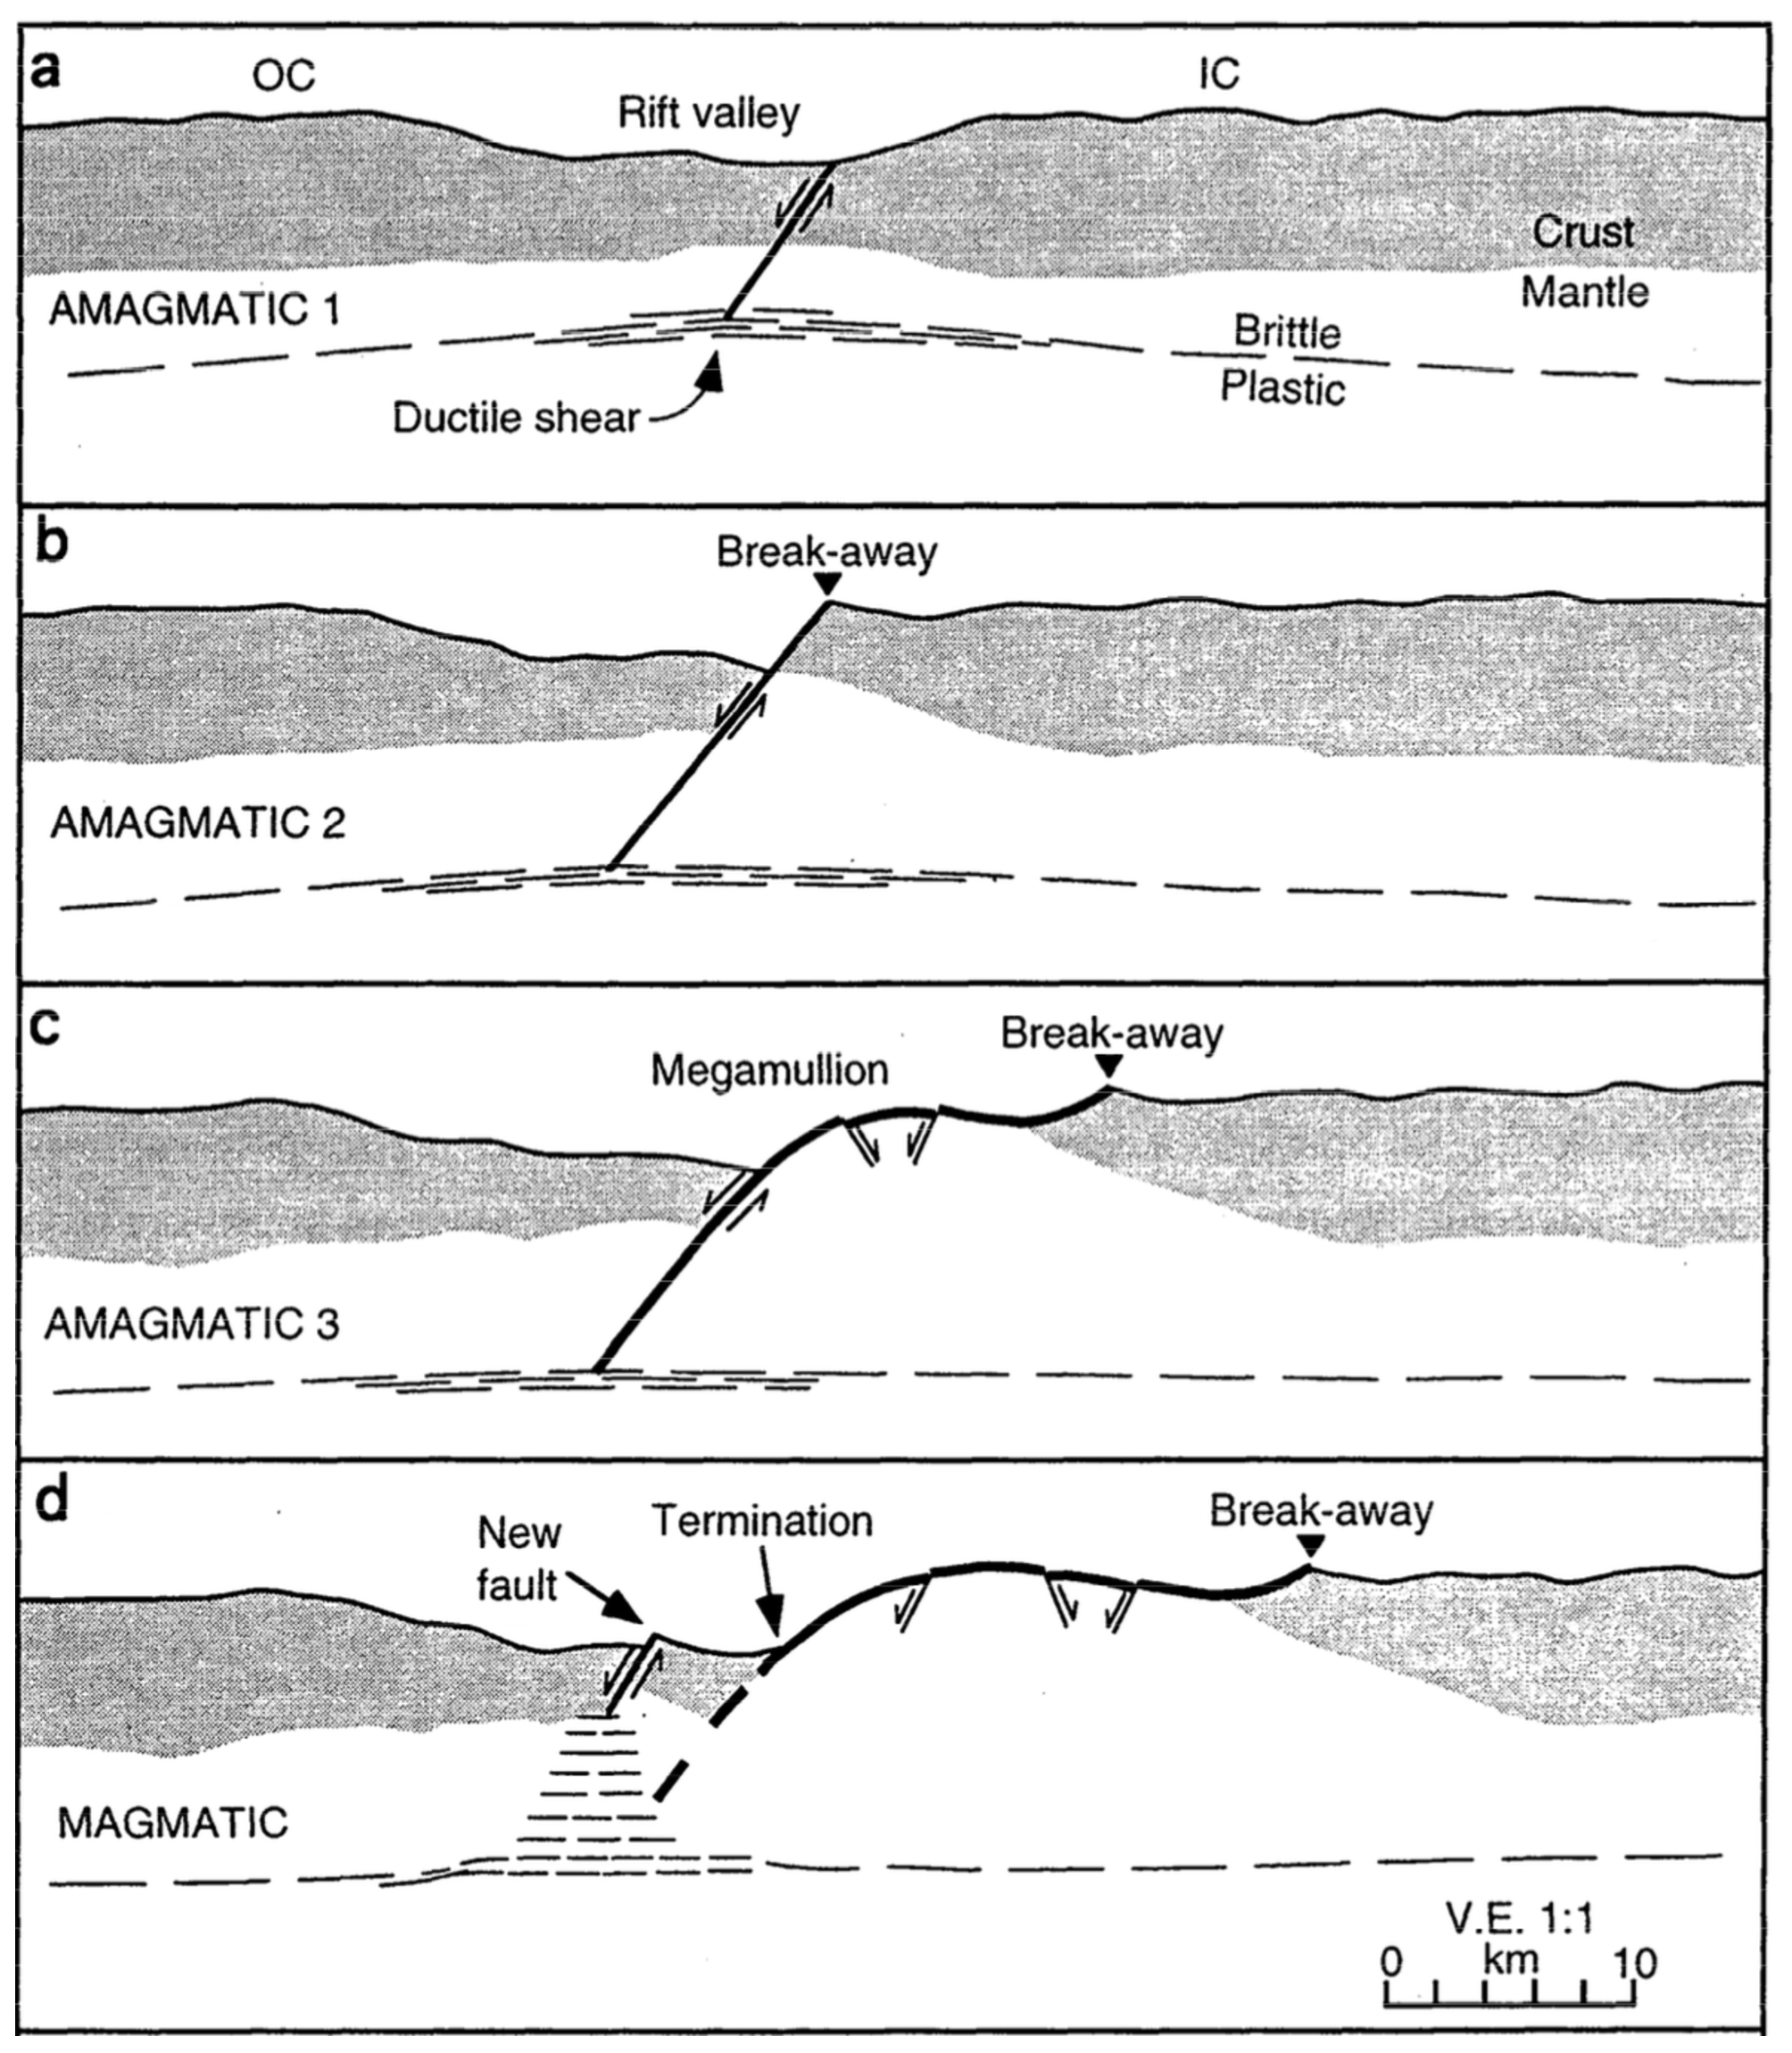
\includegraphics[width=0.7\textwidth]{./Figures/fig_Discussion_Observation_1_Tucholke1998.eps}
 \caption{Schematic development of a megamullion. No vertical exaggeration. (a)$\sim$(c) shows the detachment fault evolution during amagmatic phase. (d) Increased magma supply pushed the detachment fault away from ridge axis and forms a new normal fault near the ridge axis (``inward fault jump''). Adapted from \citep{Tucholke1998}.}
 \label{fig_Discussion_Observation_1_Tucholke1998}
\end{figure}

The term ``inward fault jump'' is first suggested in a study of geological and geophysical data from the Mid-Atlantic Ridge \citet{Tucholke1998}. It is the end phase of a general evolution of an OCC as is isllustrated in Figure~\hyperref[fig_Discussion_Observation_1_Tucholke1998]{\ref{fig_Discussion_Observation_1_Tucholke1998}}. In the begining of a long amagmatic phase (Figure~\hyperref[fig_Discussion_Observation_1_Tucholke1998]{\ref{fig_Discussion_Observation_1_Tucholke1998}.a$\sim$c}) of seafloor spreading, a high angle normal fault cuts throught the brittle lithosphere and roots in the brittle-ductile transition (BDT) (Figure~\hyperref[fig_Discussion_Observation_1_Tucholke1998]{\ref{fig_Discussion_Observation_1_Tucholke1998}.a}). When the fault keeps slipping, the breakaway moves off axis and the fault begin to rotate to a lower dip angle (Figure~\hyperref[fig_Discussion_Observation_1_Tucholke1998]{\ref{fig_Discussion_Observation_1_Tucholke1998}.b}). Then, the exposed fault surface roll over and as the detachment fault keeps exhuming lower crust and upper mantle rocks, it generates a dome shape megamullion (OCC). The high angle normal faults cut the detachment fault surface where it is exposed to the seafloor is probably caused by the bending stresses during footwall roll over (Figure~\hyperref[fig_Discussion_Observation_1_Tucholke1998]{\ref{fig_Discussion_Observation_1_Tucholke1998}.c}). Then, when magma supply at the ridge center increases and pushes the detachment fault away from the ridge axis, the OCC formation is terminated by the new fault near the ridge axis which is termed as the ``inward fault jump''. As shown in the figure, initially, the footwall of this new fault is mostly composed of crust material like basalt, however, if this new fault can last a long period of time, it can also exhume lower ultramafic material.

\begin{figure}[h]
 \centering
  \includegraphics[width=1.0\textwidth]{./Figures/fig_Discussion_Observation_2_Dick2008_Kane.eps}
 \caption{Adapted from \citep{Dick2008}.}
 \label{fig_Discussion_Observation_2_Dick2008_Kane}
\end{figure}

In our model, most of the inward fault jumps last less than 5 km of plates extension before the mantle materials can be exhumed to the seafloor. However, M28LinT1 generates a inward fault jump lasts for $\sim$15 km of extension (Figure~\hyperref[fig_Discussion_Result_Summary_1_Combine_together]{\ref{fig_Discussion_Result_Summary_1_Combine_together}}) and produces a dome shape OCC ajacent to the initial one further way from the ridge axis (Figure~\hyperref[fig_Results1_1]{\ref{fig_Results1_1}.h}). This behavior might explain the formation mechanism of the brother Abel and Cain domes of the Kane megamullion at 23 $\degree$N MAR. As shown in Figure~\hyperref[fig_Discussion_Observation_2_Dick2008_Kane]{\ref{fig_Discussion_Observation_2_Dick2008_Kane}}, our model behaviors are consistent with the nature observation in terms of the breakaway and the wavelength of the domes assuming M decreases form south to north along the ridge axis. First of all, the breakway of the detachment fault is further away from the ridge axis at the northern than the sourthern end. Second, the Abel and Cain domes are larger than the Adam and Eve domes because the inward fault jump lasts longer at where M is relatively lower.    

\begin{figure}[h]
 \centering
  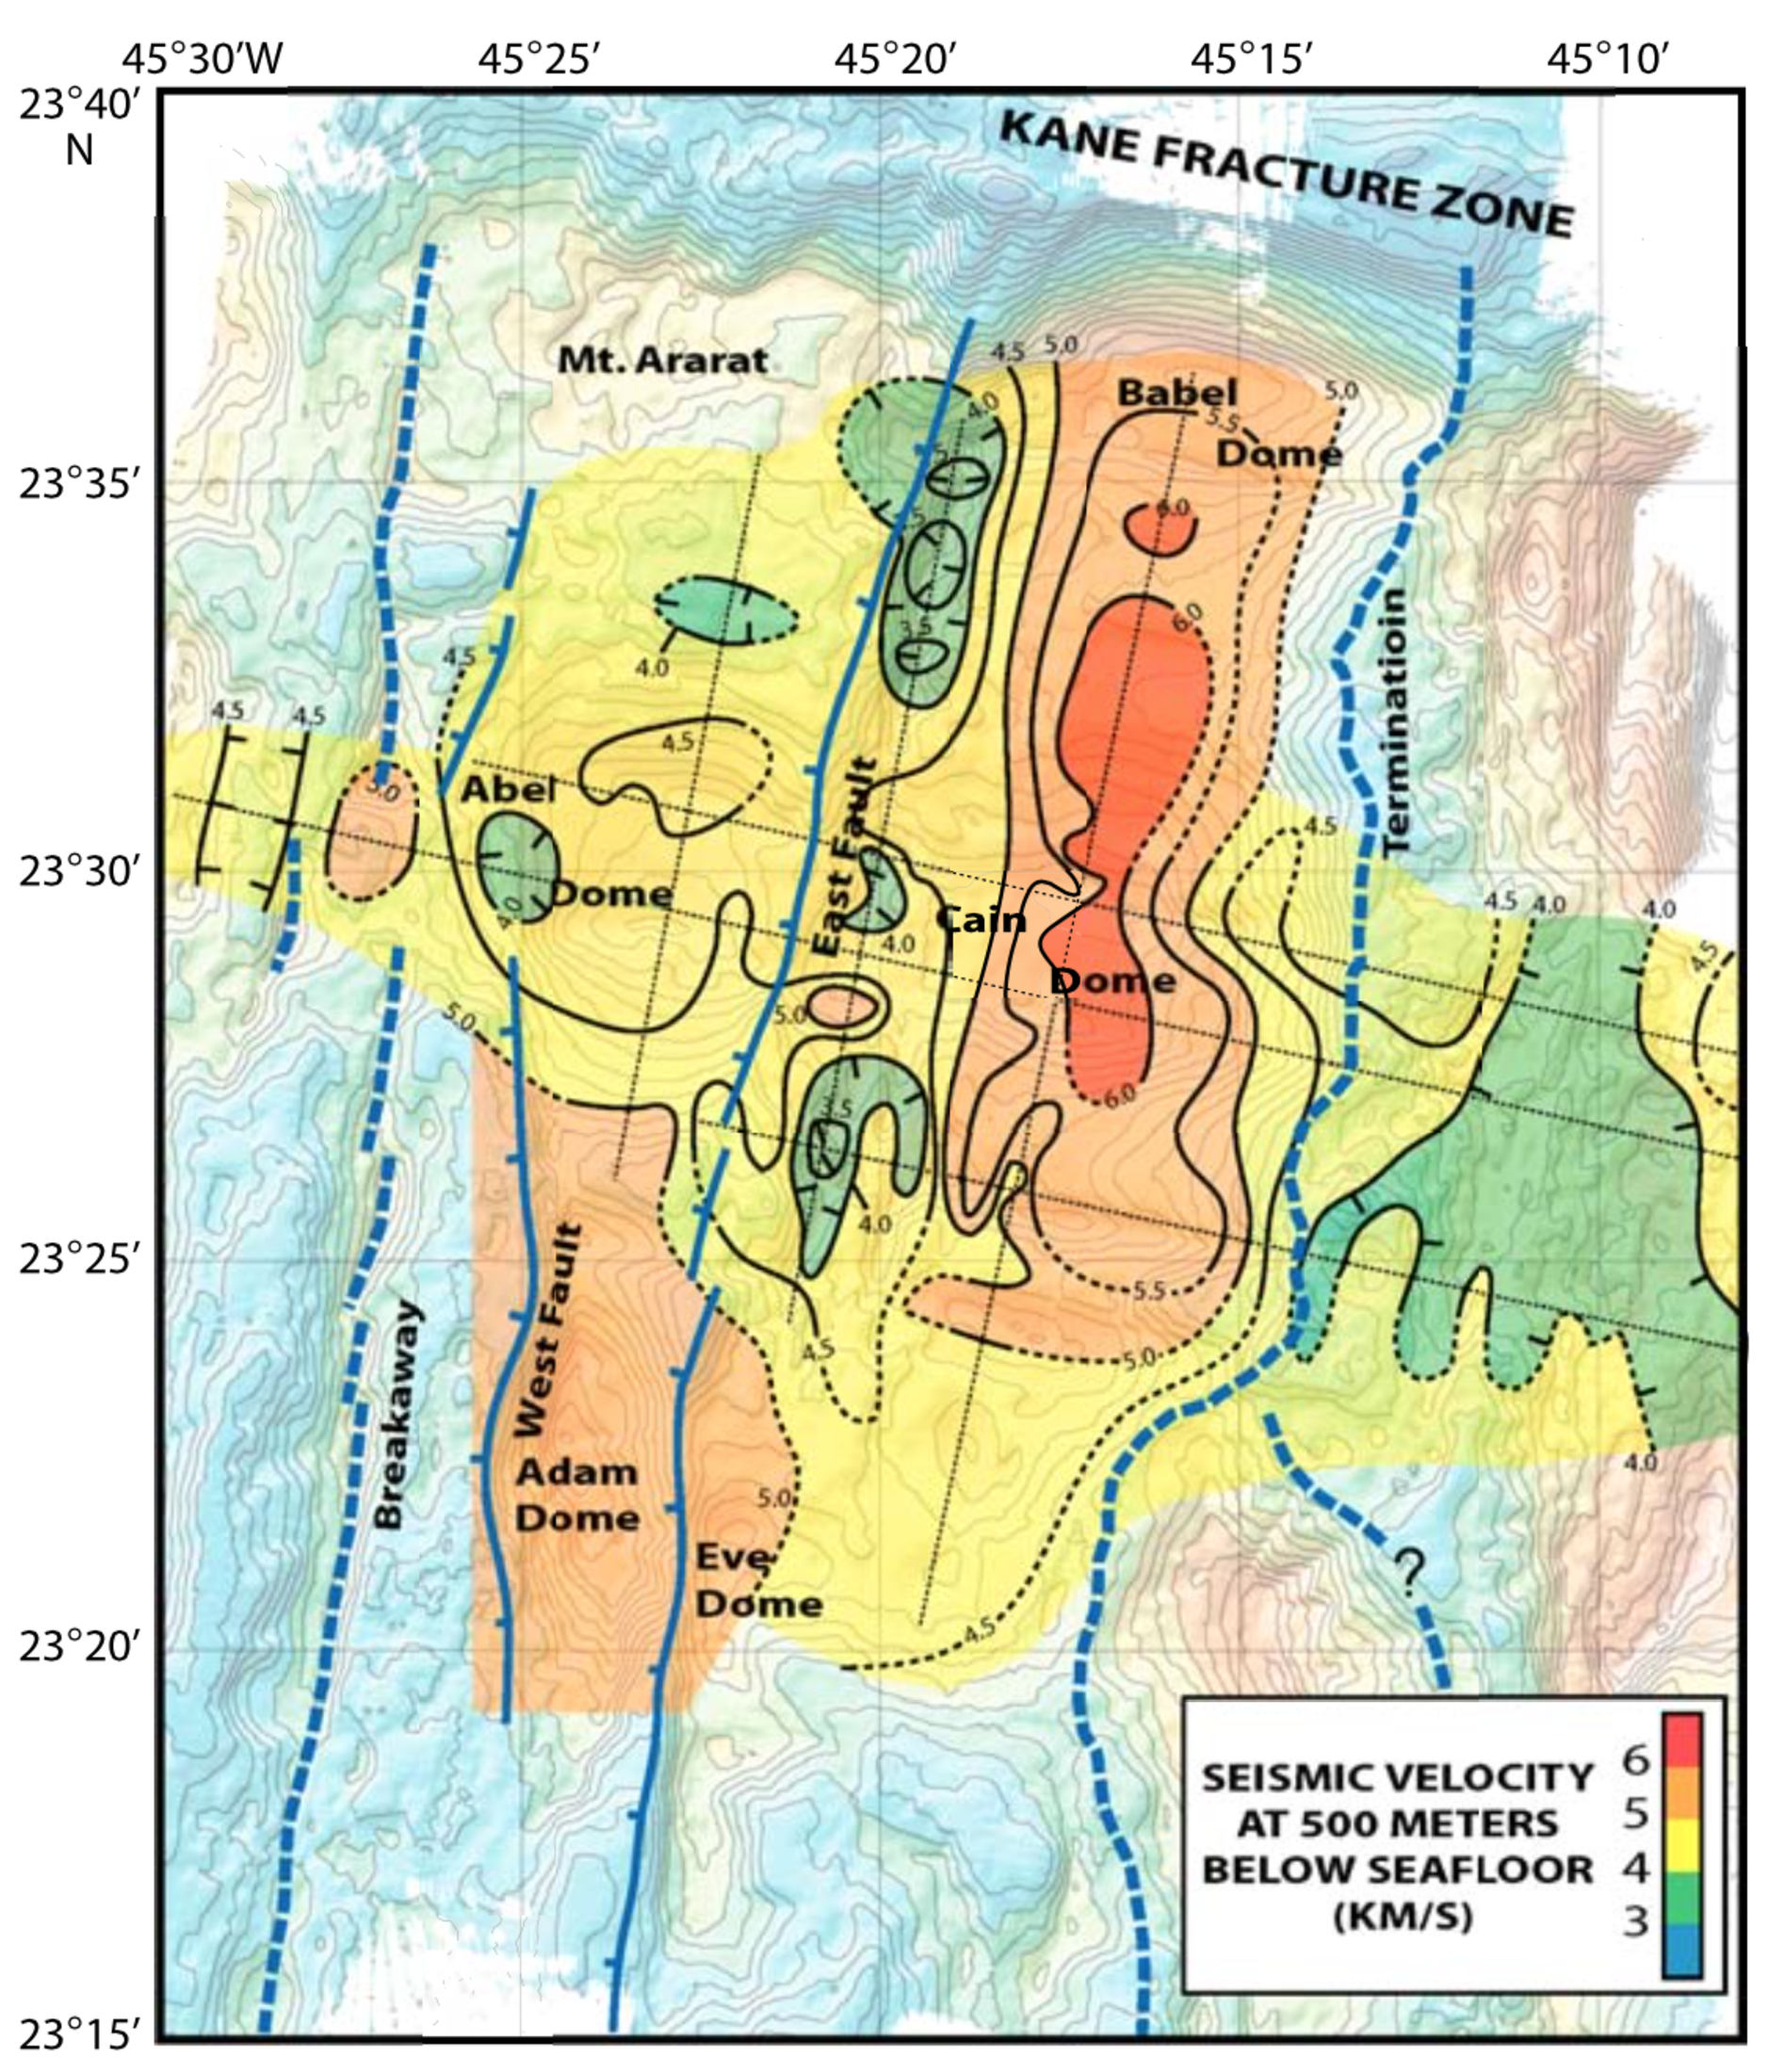
\includegraphics[width=0.6\textwidth]{./Figures/fig_Discussion_Observation_1_Xu2009_SeismicV_Kane.eps}
 \caption{Adapted from \citep{Xu2009}.}
 \label{fig_Discussion_Observation_1_Xu2009_SeismicV_Kane}
\end{figure}

In addition, it is mentioned by a seismic study from \citep{Xu2009} that the Kane OCC is terminated at around 2.1 Myr when an eastward fault jump occured, i.e. when a new normal fault formed in the rift valley and captured a segment of the basaltic hanging wall. The velocity structure from their P wave tomography study also reveals that the eastern block of the Cain dome has a lower velocity corresponds to basaltic rocks (Figure~\hyperref[fig_Discussion_Observation_1_Xu2009_SeismicV_Kane]{\ref{fig_Discussion_Observation_1_Xu2009_SeismicV_Kane}}).

\subsubsection{Fault alternation}

\begin{figure}[h]
 \centering
  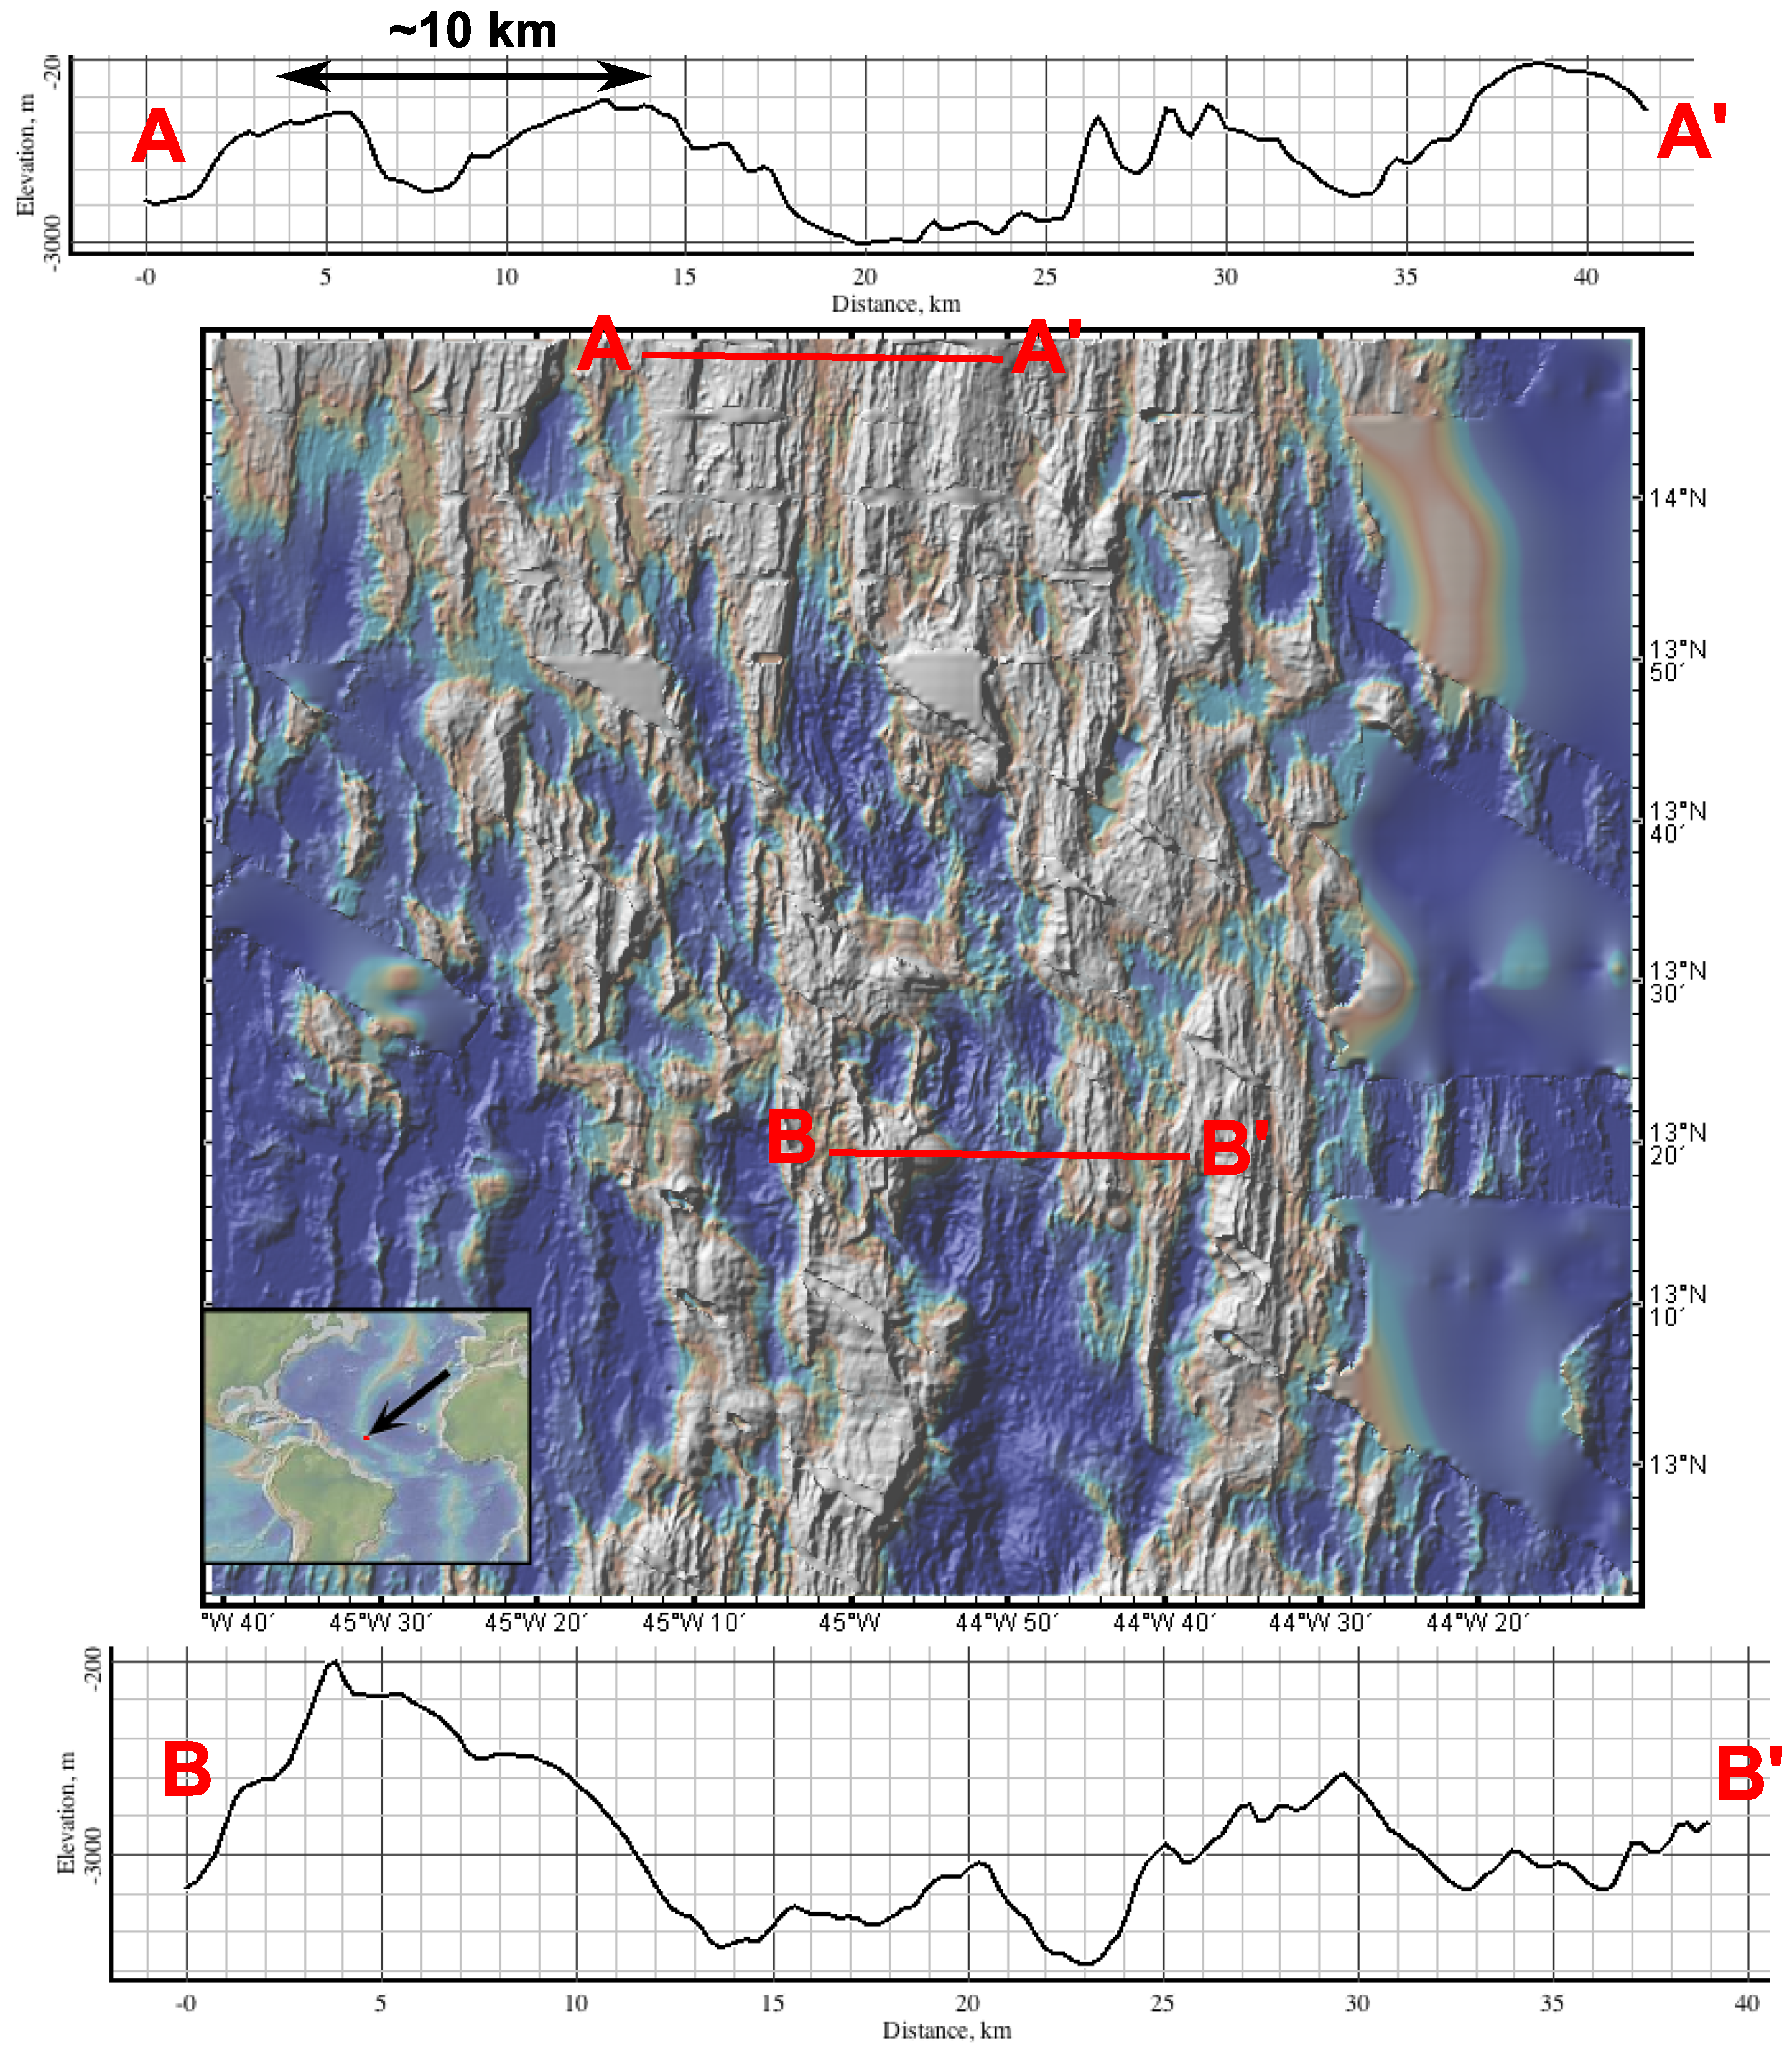
\includegraphics[width=0.75\textwidth]{./Figures/fig_Discussion_Observation_2_13-14N_MAR.eps}
 \caption{Bathymethry from 12.8$\sim$14.2 $\degree$N Mid-Atlantic Ridge. Crossection A$\sim$A$^{\prime}$ and B$\sim$B$^{\prime}$ are 5 times vertical exagerated. From GeoMapApp.}
 \label{fig_Discussion_Observation_2_13-14N_MAR}
\end{figure}

For slow-to-intermediate spreading ridges, two end members govern the off axis morphologies. One is the higher frequency symmetrically spreading abyssal hills which usually is closer to the ridge segment center (crossection A$\sim$A$^{\prime}$ in Figure~\hyperref[fig_Discussion_Observation_2_13-14N_MAR]{\ref{fig_Discussion_Observation_2_13-14N_MAR}}). The other is longer wavelength asymmetrically spreading OCCs (crossection B$\sim$B$^{\prime}$ in Figure~\hyperref[fig_Discussion_Observation_2_13-14N_MAR]{\ref{fig_Discussion_Observation_2_13-14N_MAR}}). What is the mechanism for this distinct difference along the ridge? The fault alternation behavior in our model provides a 3D perspective for answering the question. When average M $\bar{M}$ is higher than 0.6425 with slower weakening rate (type 2), high frequency abyssal hills are generated. For example, M88ConT2 produces abyssal hills with $\sim$10 km in wavelength due to fault alternation (Figure~\hyperref[fig_Discussion_Result_Summary_1_Combine_together]{\ref{fig_Discussion_Result_Summary_1_Combine_together}}). Note that the wavelength of the abysall hills in our models is consistent with the nature observation as marked in Figure~\hyperref[fig_Discussion_Observation_2_13-14N_MAR]{\ref{fig_Discussion_Observation_2_13-14N_MAR}}. 

\begin{figure}[h]
 \centering
  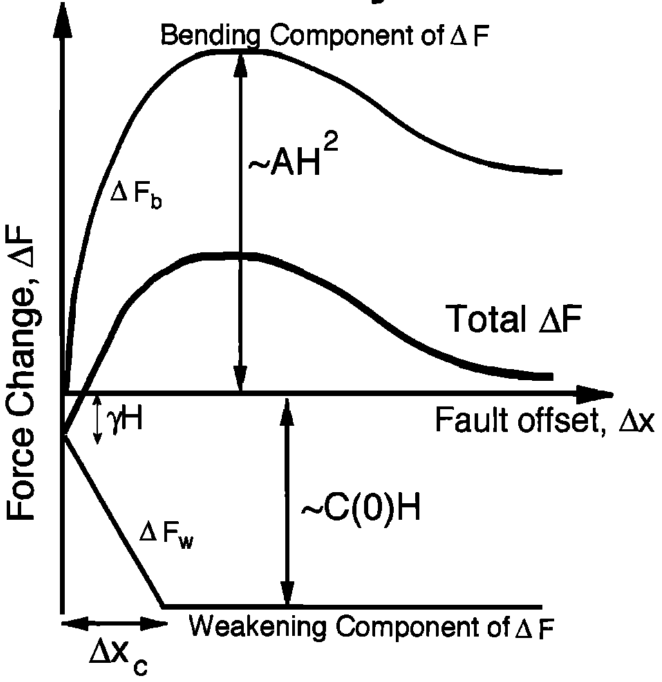
\includegraphics[width=0.45\textwidth]{./Figures/fig_Results_Weakening_1_tradeOff_bend_weak.png}
 \caption{Trade-off between change in bending force $\Delta F_{b}$ and weakening in the fault interface $\Delta F_{w}$. H is the thickness of the brittle crust and $\gamma$ is the size of initial weak perturbation and A defines the maximum bending force change. (For more details, please refer to \citep{Lavier2000})}
 \label{fig_Results_Weakening_1}
\end{figure}

The parameters that controls fault alternation is studied by \citep{Lavier2000}. There is a trade-off between change in bending force $\Delta F_{b}$ as a function of fault offset $\Delta X$ and force change $\Delta F_{w}$ as a function of  $\Delta X$ due to strain weakening. As described in \citep{Lavier2000}, higher characteristic fault offset ($\Delta X_{c}$) or slower strain weakening results in multiple faults rather than only one fault lasting. Whether conjugate fault and even multiple faults can be produced depends on the local stress condition. The strength weakening of the existed fault combines with how much bending force resists the fault to keep offseting play a major role in determining the stress state at the other areas. As the sea-floor keeps spreading and  $\Delta X$ increasing, the change in bending force $\Delta F_{b}$ increases and the strength at the fault interface decreases due to weakenging $\Delta F_{w}$ (Figure~\hyperref[fig_Results_Weakening_1]{\ref{fig_Results_Weakening_1}}). If the net force change $\Delta F = \Delta F_{b}+ \Delta F_{w}$ is positive, it means that it is getting harder and harder to maintain the existing fault and stress will begin to accummulate at the other areas which eventually break another fault. $\Delta F_{b}$ initially increases fast with respect to $\Delta X$ and then when the detachment fault surface roll over, $\Delta F_{b}$ reaches its peak value and begins to decrease a little and maintains at a constant value. If the strain weakenging is fast enough that the net effect force $\Delta F$ is always negative, then most of the stress will be released by the existing fault and thus no conjugate or multiple faults will be created. 

Our model results verify this analysis that only Type two weakening (slower weakening with higher $\Delta X_{c}$) can produce an alternating normal fault on the conjugate plate.

%Based on the previous experience in pseudo-2D models and \citep{Lavier2000},  when M$>0.5$, the frequency of normal faulting alternation is higher for higher characteristic fault offset ($\Delta X_{c}$) of Type two weakening compared to Type one weakening. However, for the reference model two, M88ConT2 (Table~\hyperref[Tab1_1]{\ref{Tab1_1}}), interesting enough, when comparing pseudo-2D and 3D models with Type two weakening under case of M$=0.8$, even though the 3D Model has a larger $\Delta X_{c}$ of 1km than that of pseudo-2D model of 0.5kmr, the 3D model M88ConT2 has a lower frequency of faulting alternation. Since M is constant 0.8 along the ridge-axis, the effect of along ridge couplingthat resists alternation need not be considered. One possibility is that the resisting bending force increase in a higher rate than linear with respect to increasing the length of the ridge segment (Z$_{max}$ km).  

\subsubsection{Mass wasting}

\begin{figure}[h]
 \centering
  \includegraphics[width=1.0\textwidth]{./Figures/fig_Discussion_Observation_1_13N_MAR_CutBack.eps}
 \caption{Comparing bathymetry at 13$\degree$N Mid-Atlantic Ridge to the mass wasting behavior of M28SqrtT1. The model topography is a mirror symetric flip according to the dash line, it reveals the case of M varies in a square root functional form from 0.2 to 0.8 to 0.2. The bathymetry image is generated by GeoMapApp \citep{Ryan2009}.}
 \label{fig_Discussion_Observation_1_13N_MAR_CutBack}
\end{figure}

\begin{figure}[h]
 \centering
  \includegraphics[width=0.8\textwidth]{./Figures/fig_Discussion_Observation_3_MassWasting_13-15N_bathymetry_magnetizaion.eps}
 \caption{Bathymetry and magnetization of 13$\sim$15 $\degree$N MAR. Adapted from \citep{Smith2008}.}
 \label{fig_Discussion_Observation_3_MassWasting_13-15N_bathymetry_magnetizaion}
\end{figure}

The mass wasting behavior in M28SqrtT1 model produces a fault scarp of $\sim$1km in relief, 40km in length along the Z axis when the detachment fault roll over and the high angle fault cut the weak detachment fault surface and decouple the spreading footwall and the highly defomed fault hangingwall. The topography at 13$\degree$N Mid-Atlantic Ridge also has a fault scarp with very similar curved geometry with $\sim$1km in relief. In addition, a magnetic anomaly study of the region from \citep{Smith2008} reveals a perfect match at the 13 $\degree$ 5 $^{\prime}$N between the bathymetry and the magnetization (Figure~\hyperref[fig_Discussion_Observation_3_MassWasting_13-15N_bathymetry_magnetizaion]{\ref{fig_Discussion_Observation_3_MassWasting_13-15N_bathymetry_magnetizaion}}). It implies that the block at 13 $\degree$ 5 $^{\prime}$N ajacent to the curved fault scarp has a relative displacement toward the East and thus provides an evidence for the mass wasting behavior of the block.   

Due to the variation in diking along the ridge-axis, an hourglass shape of median valley is also produced in the model where the narrowest center corresponds to the region with higher magma supply (M=$0.8$). This hourglass shape is also frequently observed in the nature along the Mid-Atlantic Ridges \citep{Sempere1993}.
 
\subsubsection{Hourglass shape median valley}

Hourglass shape median valley is frequently observed in the nature along the slow-to-intermediate spreading ridges where the waist of the hourglass is usually narrower and shallower. For example, from an analysis of the sea beam bathymetry along the MAR between 24 $\degree$ 00 $^{\prime}$N and 30 $\degree$ 40 $^{\prime}$N \citep{Sempere1993}, nine hourglass shape valleys are identified. They share similar dimensional scale ($\sim$40 km $\times$ $\sim$40 km) with our model.

\subsubsection{Mullion structure}

\begin{figure}[h]
  \centering
    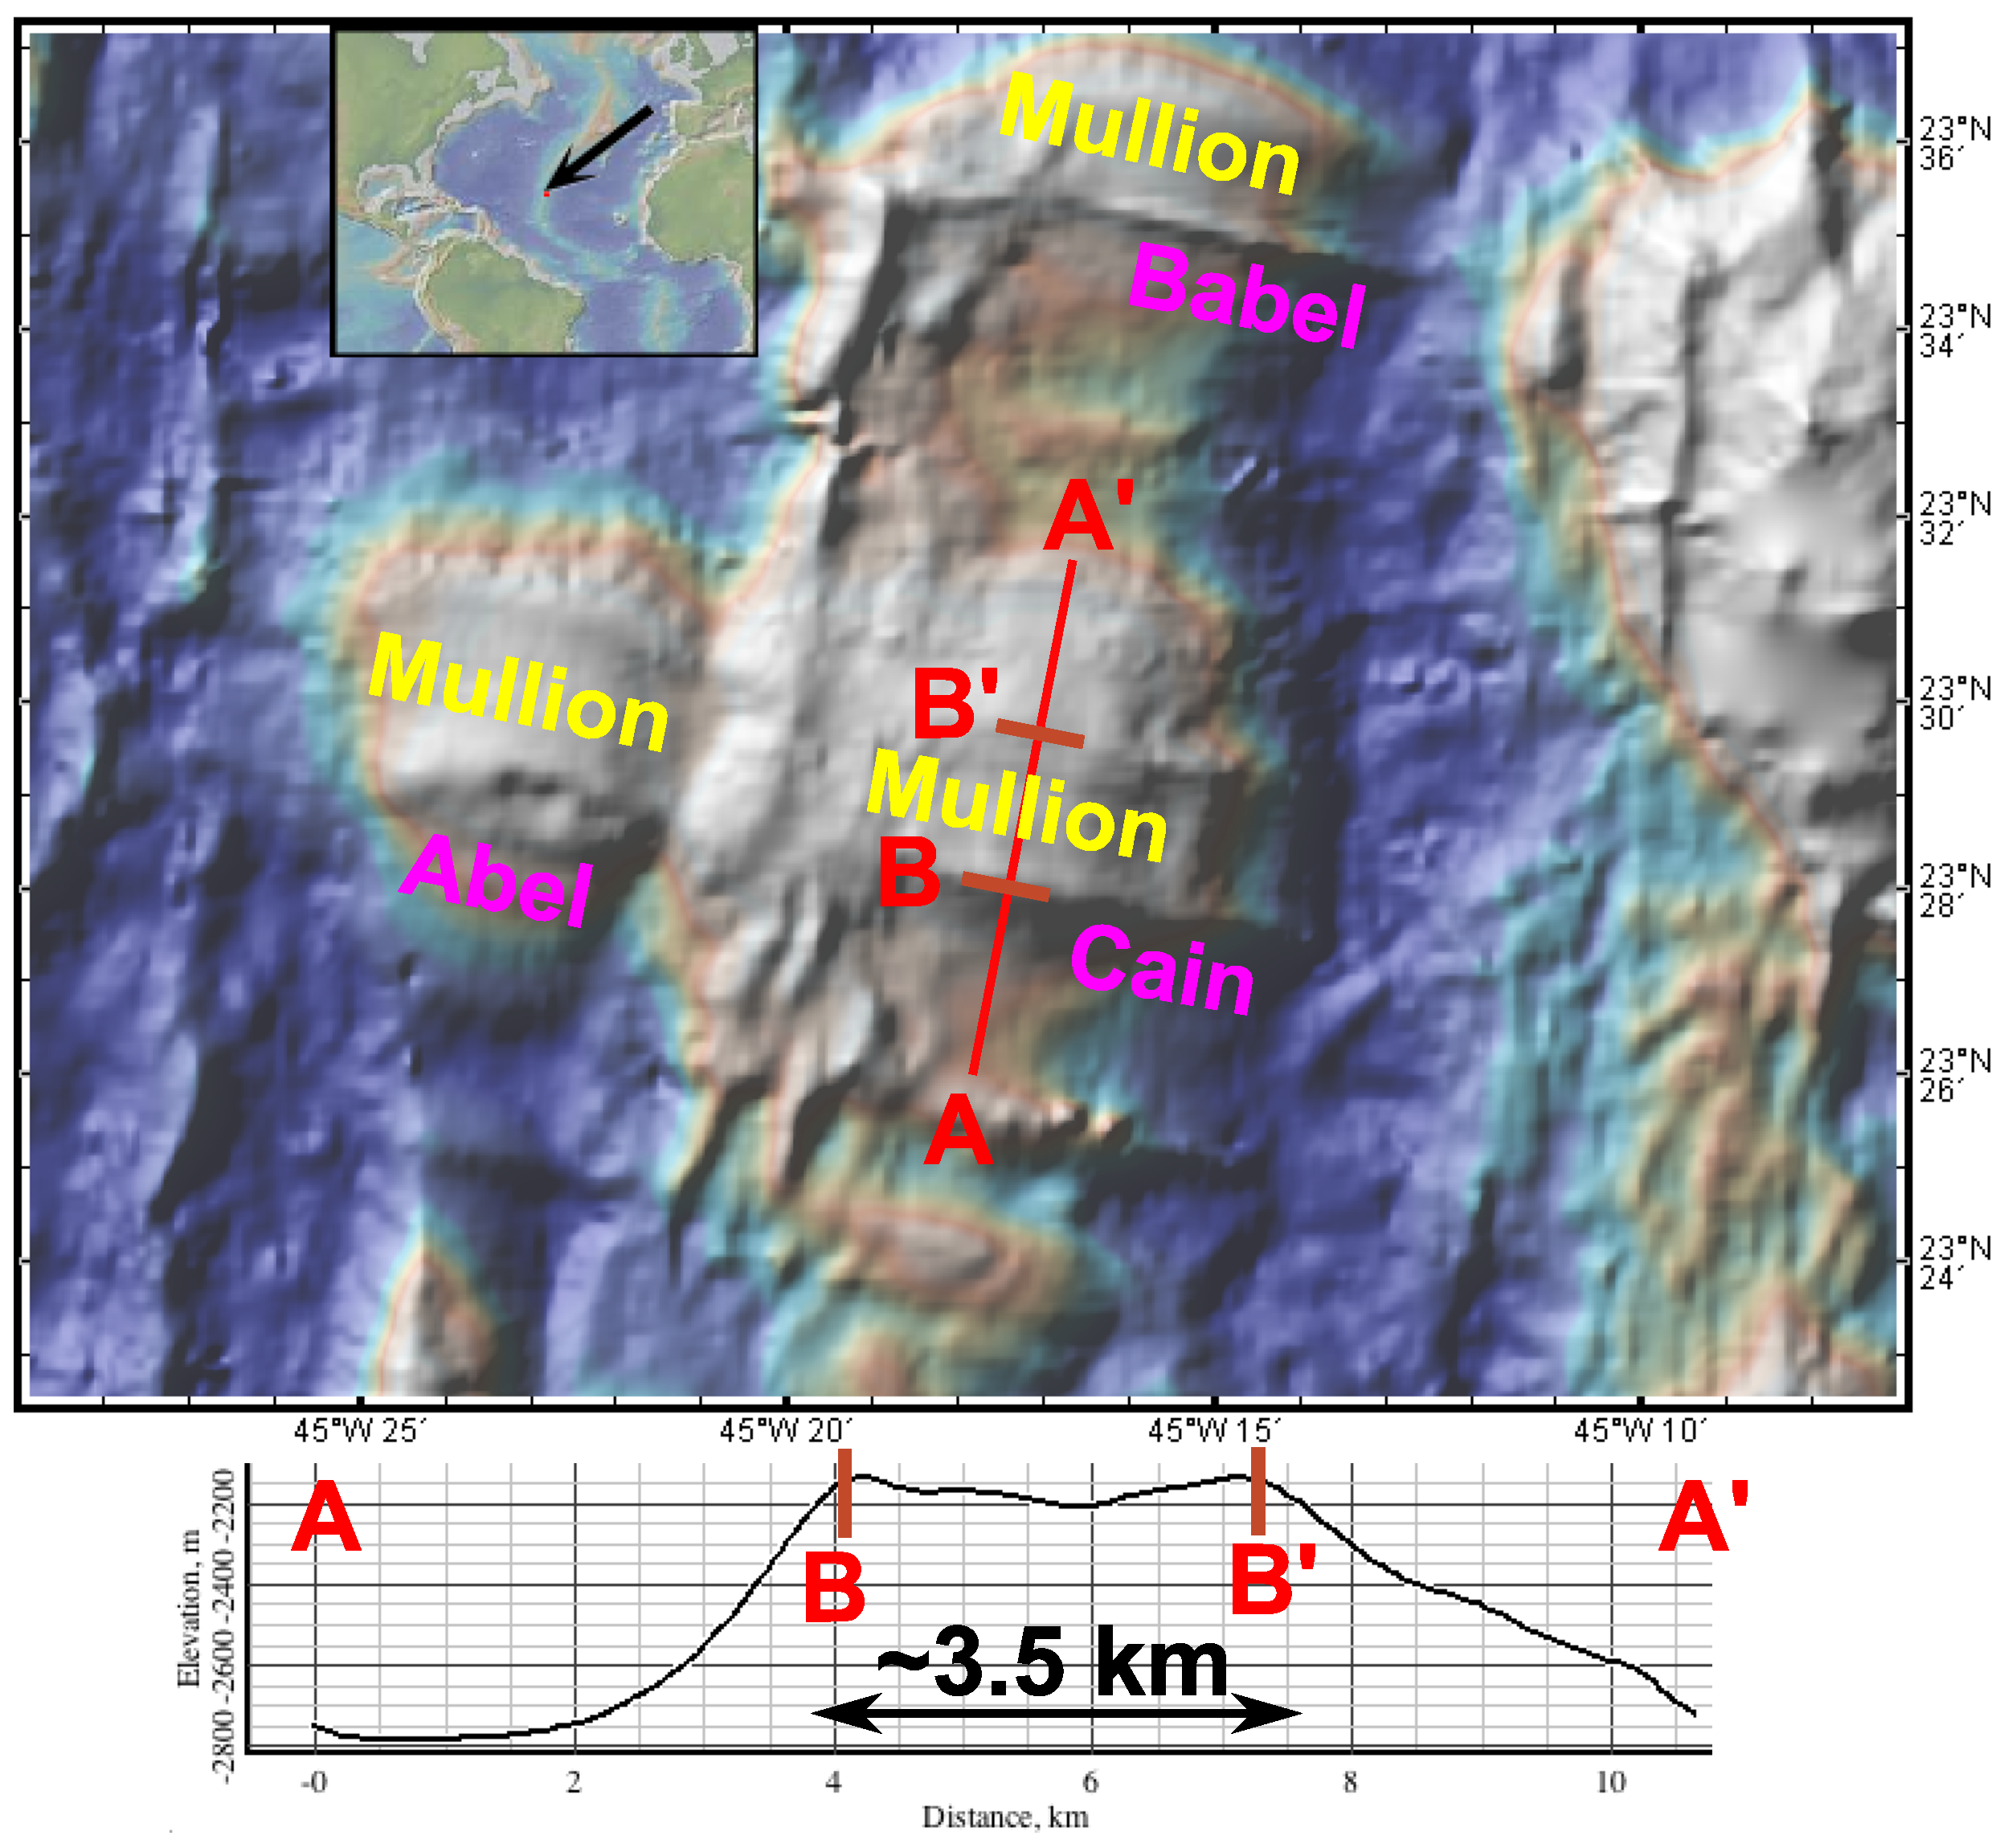
\includegraphics[width=0.8\textwidth]{./Figures/fig_Discussion_Observation_5_Mullion_Kane.eps}
  \caption{Mullion structures on the surface of Kane OCC at 23 $\degree$N MAR. Image generated from GeoMapApp.}
 \label{fig_Discussion_Observation_5_Mullion_Kane}
\end{figure}   

Mullion structure shows up frequently on the surface of OCCs. One of the most characteristic nature observation comes from Kane megamullion. The mullion structure has a wavelength of $\sim$3.5 km on the surface of of Cain dome as marked in the Figure~\hyperref[fig_Discussion_Observation_5_Mullion_Kane]{\ref{fig_Discussion_Observation_5_Mullion_Kane}}. The geometry and length scale of the mullion structure is consistenty with our model result (M28LinT1) as shown in Figure~\hyperref[fig_Results_3_2_6_mullion_evolution]{\ref{fig_Results_3_2_6_mullion_evolution}}. Model results indicate that the mullion structure is mosly formed when the termination has a curved shape that can last for long enough time. The spreading parallel mullion structure is produced following the shape of the termination. Where the termination is curved toward the ridge axis corresponds to the higher part of the mullion structure.

\subsubsection{Corrugations}



\iffalse
\subsection{Parallel computing efficiency}
\subsection{Influence of healing}
\subsection{Model Limitation}
\subsubsection{Fixed thermal structure effects and justification}
Thermal conduction rate for $\kappa=6mm^{2}/s$ material is 1.8e5 km/Myr, four magnitude faster compared to spreading rate of 2.5km/Myr.
\subsection{Recommendation for Future Research}
\fi

\iffalse
\subsection{Cut Back}\label{Sec_CutBack}

\begin{figure}[h]
  \centering
    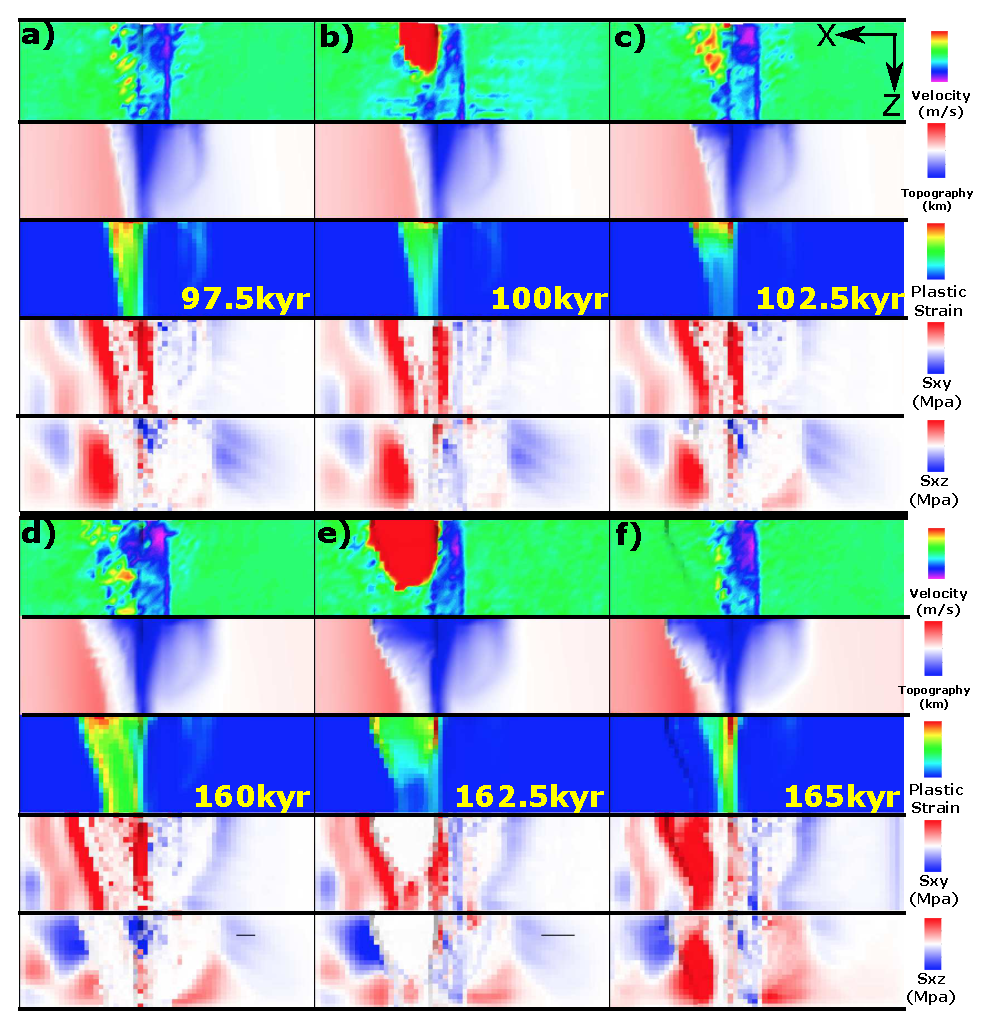
\includegraphics[width=0.8\textwidth]{./Figures/fig_Results4_4_sqrt_cut_back_with_time.eps}
  \caption{M28SqrtT1 (Table~\hyperref[Tab1_1]{\ref{Tab1_1}}). Cut back behaviors in square root functional form model with different time.}
 \label{fig_Results4_4}
\end{figure}   

\begin{figure}[h]
  \centering
    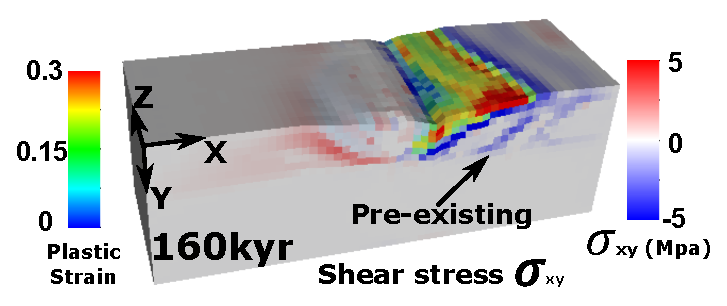
\includegraphics[width=0.6\textwidth]{./Figures/fig_Results4_5_sqrt_cut_back_pre_accummulated_shear_zone.eps}
  \caption{M28SqrtT1 (Table~\hyperref[Tab1_1]{\ref{Tab1_1}}). Square root functional form model at 160kyr. Pre-accummulated shear zone increase the shear force and cut the weak detachment front tip}
 \label{fig_Results4_5}
\end{figure}   

The cut back happens mostly in the square root model. Since the linear model and the square root model have more obvious difference in terms of the cut back behavior, here, we only compare linear and square root. There are several factors contribute to the cut back behavior. First, at the higher M side, the amount of diking for the square root model is ubiquitously larger than that of the linear one (Figure~\hyperref[fig_Results3_1]{\ref{fig_Results3_1}}). This leads to a slower bending detachment at the high M side for the square root model. Second, the totoal length of the ridge segment with M$>0.5$ for the square root model is also longer than that of the linear one (Figure~\hyperref[fig_Results3_1]{\ref{fig_Results3_1}}). This results in that at the low M side, $\sigma_{xz}$ is focused at low Z ajacent to the ridge-axis (Figure~\hyperref[fig_Results4_3_1]{\ref{fig_Results4_3_1}.e}), however for linear is spread out to Z higher than 10. Third, due to higher value of $\frac{dM}{dZ}$ for square root when Z$<5$, the along ridge-axis shear $\sigma_{xz}$ for square root will be accummulating faster, which produces larger strike-slip force to cut the hanging wall at the low M side. Fourth, as observed in the model (Figure~\hyperref[fig_Results4_3_1]{\ref{fig_Results4_3_1}.c}), the parallel to spreading direction offset between breakaways along the ridge-axis is 4km for the square root model compared to 3km for the linear model. This causes the square root model to experience bigger shear stress $\sigma_{xy}$ both immediately beneath and above the fault interface at the low M side (Figure~\hyperref[fig_Results4_3_1]{\ref{fig_Results4_3_1}.d}). Fifth, as shown in Figure~\hyperref[fig_Results4_8]{\ref{fig_Results4_8}}, due to bending of the crust at the footwall side, below the blue neutral plane, $\sigma_{xx}>0$, meaning tensional stress being accummulated as fault develops. The resulting force tends to unbend the bent crust and drag down the connecting surface (the future decoupled hanging wall). All five factors together assist in the decouple of the hanging wall at the low M side as described in detail in the next paragraph.

\begin{figure}[h]
  \centering
    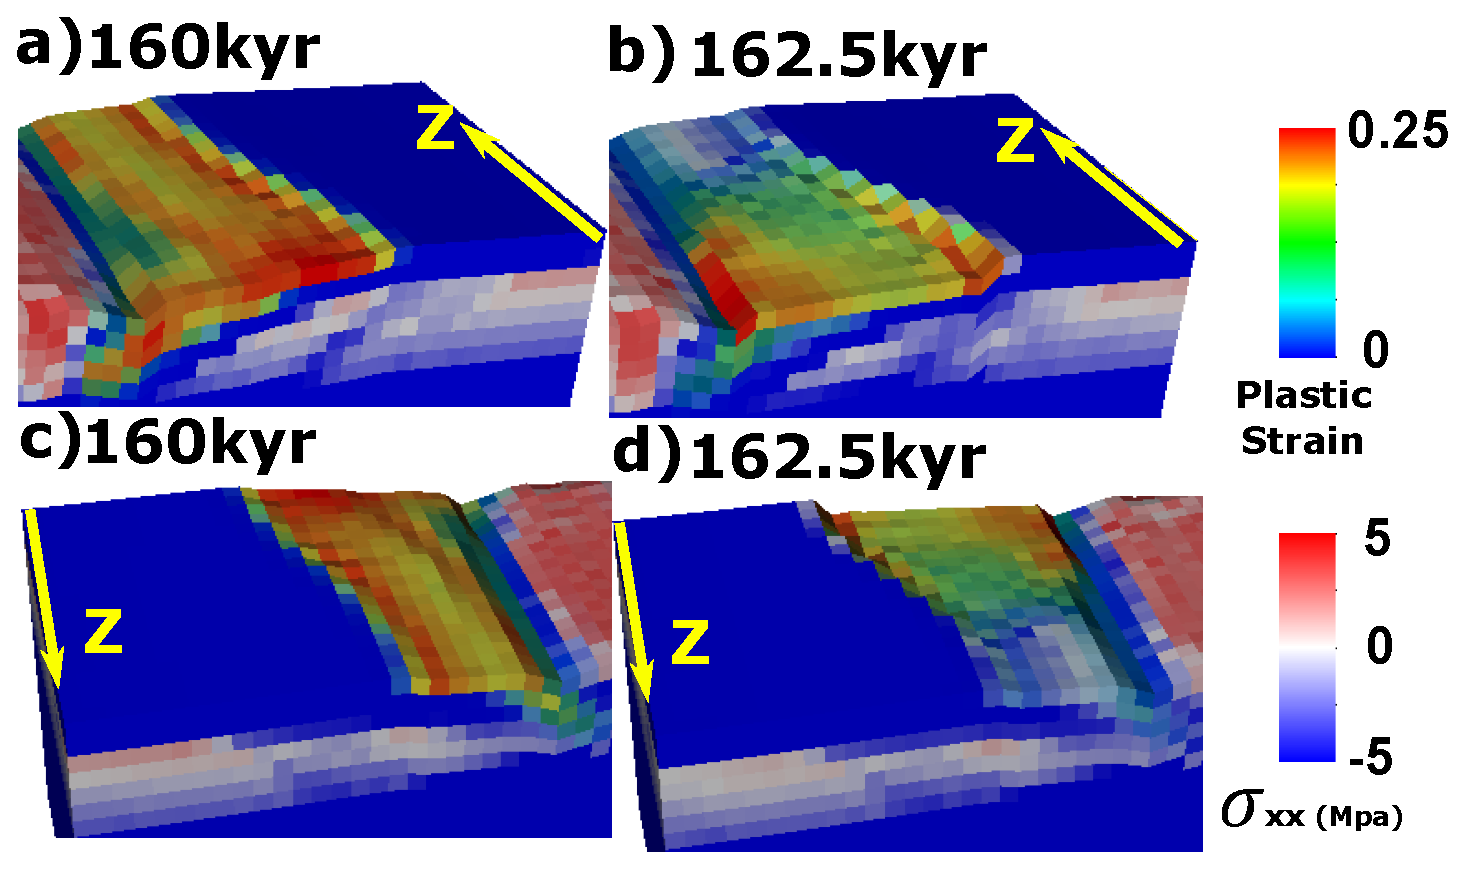
\includegraphics[width=0.6\textwidth]{./Figures/fig_Results4_6_sqrt_cut_back_bending_drop.eps}
  \caption{M28SqrtT1 (Table~\hyperref[Tab1_1]{\ref{Tab1_1}}). Bending stress drop in the crust close to dike due to cut back behavior.}
 \label{fig_Results4_6}
\end{figure}

%(Figure~\hyperref[fig_Results4_6]{\ref{fig_Results4_6}})reveals that
In the Figure~\hyperref[fig_Results4_4]{\ref{fig_Results4_4}}, the hanging wall rebounds backwards to the dike in a high velocity (Figure~\hyperref[fig_Results4_4]{\ref{fig_Results4_4}.b,e (velocity)}) accompanied with a sudden topography drop (Figure~\hyperref[fig_Results4_4]{\ref{fig_Results4_4}.b) compared to c); d) compared to e) (in the second row)}). This behavior is triggered when the front tip of the weak detachment extends further away from the ridge-axis and reaches a pre-accummulated shear zone (Figure~\hyperref[fig_Results4_5]{\ref{fig_Results4_5}}). The pre-accummulated shear zone adds extra shear force to the weak (Figure~\hyperref[fig_Results4_4]{\ref{fig_Results4_4}}.d(third row: plastic strain)) as well as shear stresses accummulated (Figure~\hyperref[fig_Results4_4]{\ref{fig_Results4_4}.d}(fourth and fifth row: $\sigma_{xy}$ and $\sigma_{xz}$)) fault interface and together with the five factors mentioned in the previous paragraph result in the cut back behavior. The cut back produces a continuous high angle fault scarp with a relief of $\sim 1km$ aligns to the initial breakaway and extends for about 20 kilometer in length (Figure~\hyperref[fig_Results4_4]{\ref{fig_Results4_4}.e (second row: topography)}). Its distance to the ridge-axis varies along the Z-axis and this result can be used to indicate the magma supply variation in the nature. \add[XT]{To be discussed in observation comparison section. as a reminder}

During the cut back process, the tensional bending stress are released at the low M side ($0<$Z$<7$) in the left tip of the bended crust (Figure~\hyperref[fig_Results4_6]{\ref{fig_Results4_6}.a compared to b}), however, in the higher M side, the tensional bending stress keeps accummulating due to the far field extension (Figure~\hyperref[fig_Results4_6]{\ref{fig_Results4_6}.c compared to d}). This behavior assists in the decouple between low M and high M side hanging walls. 

Once the cut back happens at 162.5kyr, the $\sigma_{xy}$, $\sigma_{xz}$ and $\sigma_{xx}$ are released (Figure~\hyperref[fig_Results4_4]{\ref{fig_Results4_4}.e (fourth and fifth row: $\sigma_{xy}$ and $\sigma_{xz}$)}). The plastic strain near the ridge-axis at low M side reaches a maximum of $\sim$0.9 (Figure~\hyperref[fig_Results4_4]{\ref{fig_Results4_4}.e (third row: plastic strain)}) compared to $\sim$0.3 before and after. This is due to the sudden backward motion squeezes the end element of the hanging wall near the ridge-axis and later be released by the continuous extension.

After the cut back, the termination of the detachment recedes backwards for about 7 kilometer towards the ridge-axis (Figure~\hyperref[fig_Results4_4]{\ref{fig_Results4_4}.f (third row: plastic strain)}) (termination fronts are always consistent with tension stresses in $\sigma_{xx}$ and $\sigma_{zz}$ as well as with plastic strain front(due to healing, high plastic strain region corresponds only to region with continuously deformation) (Figure~\hyperref[fig_Results4_3_1]{\ref{fig_Results4_3_1}} and Figure~\hyperref[fig_Results4_3_2]{\ref{fig_Results4_3_2}})). This behavior helps maintain a high angle normal fault. Different from the linear and sinusoidal models that the detachments at the low M side will rotate to a very low angle, square root model doesn't. In addition, $\sigma_{xy}$ and $\sigma_{xz}$ soon fill in the area between cut back created fault scarp and the new termination (Figure~\hyperref[fig_Results4_4]{\ref{fig_Results4_4}.f (fourth and fifth row: $\sigma_{xy}$ and $\sigma_{xz}$)} because $\sigma_{xy}$ always accummulates immediately beneath the normal fault interface and the red $\sigma_{xz}$ left to the new termination is due to the along ridge-axis variatioin in the rate of fault slip (low M side larger).  

\begin{figure}[h]
  \centering
    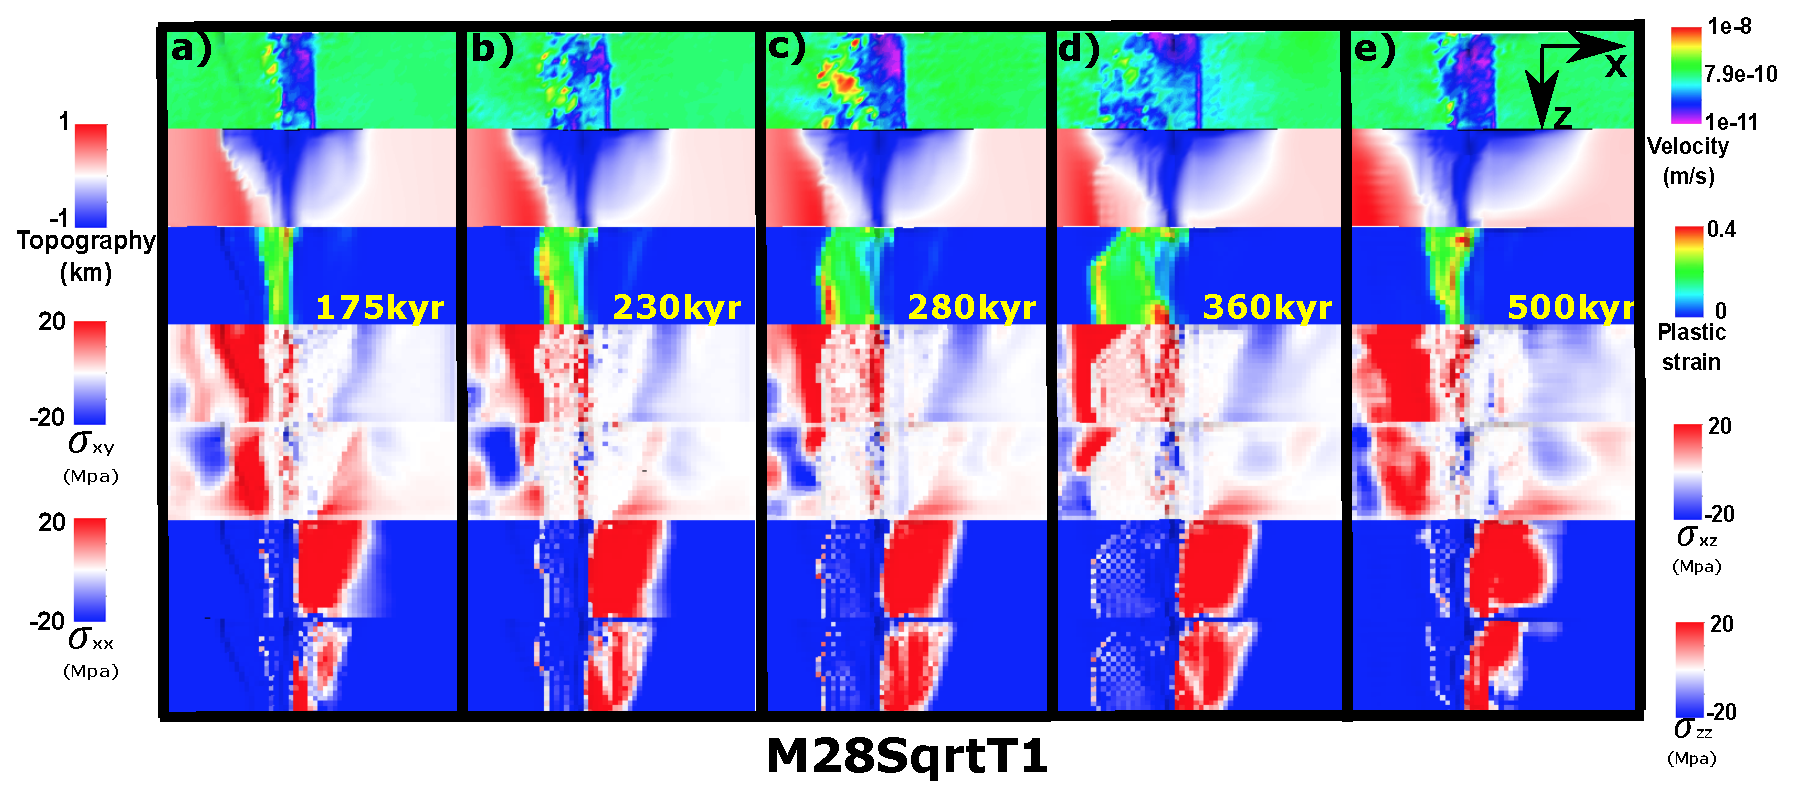
\includegraphics[width=1.0\textwidth]{./Figures/fig_Results4_9_sqrt_cut_back_new_fault_chase.eps}
  \caption{M28SqrtT1 (Table~\hyperref[Tab1_1]{\ref{Tab1_1}}). New fault front chase after initial abandoned breakaway.}
 \label{fig_Results4_9}
\end{figure}

There is one phenomenon very interesting and counter-intuitive that worth describing here. After the cut back, and termination retreat, the evolution of the detachment fronts is opposite to initiall or to the general behavior in the linear and sinusoidal models. The termination front at the high M side extends faster and further after the cut back (Figure~\hyperref[fig_Results4_9]{\ref{fig_Results4_9}}). This is partly related to the unbending decouple phenomenon we described ealier that the tensional stress are released at the low M side but continues to accummulate in the high M side during the cut back unbending in the low M side. Since the tensional stress is released in the low M side, it needs time to accummulate to where it was and then start from there to drag the new near ridge-axis fault away from the ridge-axis while at the high M side the increasing tensional stress will directly lead to a fast extending fault front. Thus create the behavior. \add[XT]{One question is, how to explain that the fault front is moving much faster than the initial abandoned breakaway? New fault front soon reach the old breakaway.} This phenomenon is largely responsible for the corrugations observed. It create a ``X'' shape ``scan'' that first ``scan'' the topography with faster low M side (Figure~\hyperref[fig_Results4_4]{\ref{fig_Results4_4}.d and e}) and then with faster high M side (Figure~\hyperref[fig_Results4_9]{\ref{fig_Results4_9}.c and d}). This results in curved terminations with hundreds to several kilometers wavelengths that directly create parallel to spreading direction corrugations.    

\begin{figure}[h]
  \centering
    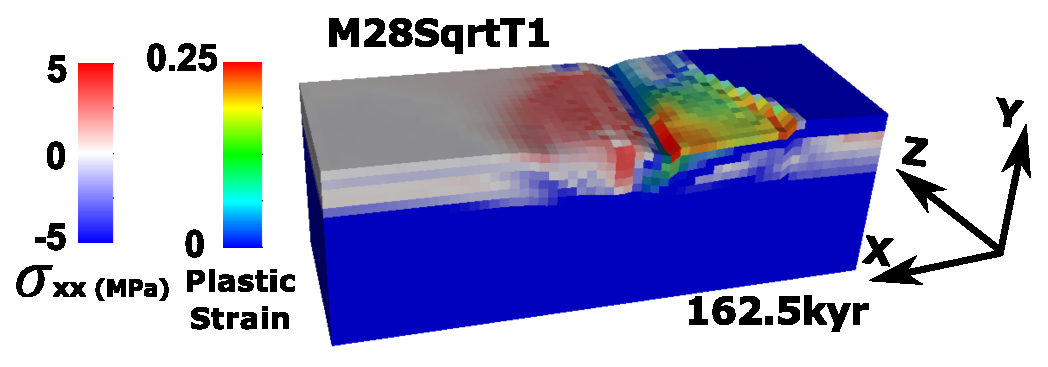
\includegraphics[width=0.6\textwidth]{./Figures/fig_Results4_7_sqrt_cut_back_conjugate_Sxx.eps}
  \caption{M28SqrtT1 (Table~\hyperref[Tab1_1]{\ref{Tab1_1}}). Higher $\sigma_{xx}$ in the median valley of conjugate plate at low M side. }
 \label{fig_Results4_7}
\end{figure}

In addition, the higher $\sigma_{xx}$ in the median valley of conjugate plate at low M side (Figure~\hyperref[fig_Results4_7]{\ref{fig_Results4_7}}) is due to the brittle crust is thinnest at the median valley, thus when same amount of force propagates from far field extension to the center median valley, the stress will increases.    
\fi



\iffalse  tables with model features
There are several behaviors that are controlled by the model parameters. Generally, only M58 models with type 2 weakening produce aternating faults on both side of the ridge axis. All the models show corrugations. As for faulting patterns in terms of evolution frequency, usually Square root is more dynamic than Sinusoidal than Linear, M58 is more dynamic than M57 than M28.

Following tables are a summery of the model behaviors with respect to different setup parameters.
 

\begin{table}[h]
\begin{small}
\begin{center}
\begin{tabular}{||l|l||l|l||l|l||}
\hline
A & Alternating Fault & C & Corrugation & SL & Shear Topography Low \\
\hline
NA& Not Alternating & SF & Secondary Fault on one side & CB & Cut Back   \\
\hline
DD &  Double Dome  & AM    & Atlantis Massif Shape &  &   \\
\hline
\end{tabular}
\end{center}
\end{small}
\caption{Model behaviors in short.}
\label{Tab1}
\end{table}

Based on the 11 models with M variation, we observed eight first-order behaviors as shown in Table~\hyperref[Tab1]{\ref{Tab1}}. 


\begin{table}[h]
\begin{small}
\begin{center}
\begin{tabular}{|l|p{3.5cm}|p{3.5cm}|p{3.5cm}|}
\hline
\diagbox[width=6em]{Type}{M range}&
M28&M57&M58\\
\hline
Type one &NA; C; SL; SF$_{1500 kyr}$; DD    &NA; C; SF$_{1380 kyr}$; CB$_{330 kyr}$; AM(opposite z)     &    \\
\hline
Type two &    &     &    \\
\hline
\end{tabular}
\end{center}
\end{small}
\caption{Linear functional form.}
\end{table}

\begin{center}
\begin{table}[h!]
\begin{small}
\begin{tabular}{|l|p{3.5cm}|p{3.5cm}|p{3.5cm}|}
\hline
\diagbox[width=6em]{Type}{M range}&
M28&M57&M58\\
\hline
Type one & NA; C; SL; SF$_{995 kyr}$ & NA; C; SL; SF$_{760 kyr;1320 kyr}$; CB$_{520 kyr}$; AM & NA; C; SL; CB$_{510 kyr}$; SF$_{760 kyr;1140 kyr;1990 kyr}$   \\
\hline
Type two &    &NA; C; SL; SF$_{680 kyr}$; CB$_{905 kyr}$     & A$_{450 kyr;600 kyr}$; C(only at low M); CB$_{990 kyr}$   \\
\hline
\end{tabular}
\end{small}
\caption{Sinusoidal functional form.}
\end{table}
\end{center}

\begin{table}[ht]
\begin{small}
\begin{center}
\begin{tabular}{|l|p{3.5cm}|p{3.5cm}|p{3.5cm}|}
\hline
\diagbox[width=6em]{Type}{M range}&
M28&M57&M58\\
\hline
Type one & NA; C; SL; CB$_{205 kyr;330 kyr;1025 kyr}$   &      & NA; C$_{1770 kyr}$(due to shear with dif wave length); SF$_{860 kyr}$(high M); SF$_{1190 kyr}$(low M)(Dog Bone); SF$_{1690 kyr}$    \\
\hline
Type two &    & NA; C; SF$_{435 kyr;1060 kyr}$; CB$_{585 kyr}$; CB$_{735 kyr}$; CB$_{910 kyr}$; CB$_{970 kyr}$    & A$_{550 kyr;920 kyr}$; C; CB$_{400 kyr}$    \\
\hline
\end{tabular}
\end{center}
\end{small}
\caption{Square root functional form.}
\end{table}

Generally, all models forms a median valley that deepens and widens toward the lower M side (Figure~\hyperref[fig_Results1_1]{\ref{fig_Results1_1}}) except the reference model with constant M$=0.8$ (Figure~\hyperref[fig_Results1_3]{\ref{fig_Results1_3}}). The topography oberseved in our models, to the first order, is controlled by the spatial and temporal distributions of faulting and to the second order, results from elastically deformation (e.g. The gradual deepening and widening of the median valley; The bending of the crust at the footwall side of the detatchment fault results in a domal shape of the fault interface as a mechanism for producing the dome shape of OCCs). 

The pattern of the deformation (faulting and elastic deformation) is controlled by the evolving stress in the crust in terms of its distribution and magnitude. The stress evolution is a result of the interaction processes between tectonics and magmatism. Due to constant seafloor spreading, tensional stress orthogonal to the ridge-axis in the crust keeps accummulating. At the same time, along ridge-axis varying diking partially accommodates the stress from far field extension and perturbs the homogeneity state of stress distribution along the ridge-axis. Accumulated stress will be largely released when the tensile or shear failures establish.

Since the model behavior is very complicated. We will focus on the effects being brought by the along ridge-axis variation in diking. Thus, it is worth considering a thought experiment with two end members: One, the along ridge-axis coupling is rigid, so that even along ridge axis variation in M exist, once a fault determined to develop, it will cut through the whole model domain along the ridge-axis(Z-axis) simultaneously. The other end member is that there is totally no coupling along the ridge-axis. So that each slice of crossection profile across the ridge behave separately without being influenced by its neighbour to a extreme that the model behavior is just a combination of 20 pseudo-2D models piled up along ridge-axis with their own M. (IMPORTANT: this suggests the importance and urgence for making clear conclusion and results description for previous pseudo-2D models results. However, one difficulty here is that the characteristic fault offset $\Delta X_{c}$ is different between 2D and 3D models.)
\fi
